% --------------------------------------------------------
% DEFINIÇÕES DO DOCUMENTO
% --------------------------------------------------------

\documentclass[
	% -- opções da classe memoir --
	12pt,				% tamanho da fonte
	openright,			% capítulos começam em pág ímpar (insere página vazia caso preciso)
	oneside,			% para impressão em verso e anverso. Oposto a twoside
	a4paper,			% tamanho do papel.
	% -- opções da classe abntex2 --
	%chapter=TITLE,		% títulos de capítulos convertidos em letras maiúsculas
	%section=TITLE,		% títulos de seções convertidos em letras maiúsculas
	%subsection=TITLE,	% títulos de subseções convertidos em letras maiúsculas
	%subsubsection=TITLE,% títulos de subsubseções convertidos em letras maiúsculas
	% -- opções do pacote babel --
	english,			% idioma adicional para hifenização
	french,				% idioma adicional para hifenização
	spanish,			% idioma adicional para hifenização
	brazil,				% o último idioma é o principal do documento
	]{lib/abntex2}


% --------------------------------------------------------
% PACOTES
% --------------------------------------------------------
\usepackage{cmap}				% Mapear caracteres especiais no PDF
\usepackage{lmodern}			% Usa a fonte Latin Modern
\usepackage[T1]{fontenc}		% Selecao de codigos de fonte.
\usepackage[utf8]{inputenc}		% Codificacao do documento (conversão automática dos acentos)
\usepackage{lastpage}			% Usado pela Ficha catalográfica
\usepackage{indentfirst}		% Indenta o primeiro parágrafo de cada seção.
\usepackage{color}				% Controle das cores
\usepackage{graphicx}			% Inclusão de gráficos
\usepackage{lipsum}				% para geração de dummy text
\usepackage{float}

%\usepackage{caption}
%\captionsetup[table]{name=Quadro}

\let\printglossary\relax
\let\theglossary\relax
\let\endtheglossary\relax
\usepackage{lib/update-abntex}

\usepackage{gensymb}

\usepackage[brazilian,hyperpageref]{}	 % Paginas com as citações na bibl
\usepackage{microtype} 

\usepackage{silence}
%Disable all warnings issued by latex starting with "You have..."
\WarningFilter{latex}{You have requested package}
\usepackage[alf, abnt-etal-list=0 ]{lib/abntex2cite}	% Citações padrão ABNT
\usepackage[br]{lib/nicealgo}       % Pacote para criação de algoritmos
\usepackage{lib/customizacoes}      % Pacote de customizações do abntex2

\usepackage{listings}
\usepackage[normalem]{ulem} % Strikethrough package
\usepackage[tablename=Quadro]{caption}

% --------------------------------------------------------
% CONFIGURAÇÕES DE PACOTES
% --------------------------------------------------------

% Configurações do pacote listing
\renewcommand{\lstlistingname}{Código} %Mudança no caption do listing para Código
\renewcommand{\lstlistlistingname}{Lista de códigos} %Mudança no caption da lista de listings.

% Contagem de códigos sem incluir o número do capítulo
\usepackage{chngcntr}
\AtBeginDocument{\counterwithout{lstlisting}{chapter}}


% Configurações do pacote backref
\renewcommand{\familydefault}{\sfdefault}
% Usado sem a opção hyperpageref de backref
% \renewcommand{\backrefpagesname}{Citado na(s) página(s):~}
% Texto padrão antes do número das páginas
% \renewcommand{\backref}{}
% Define os textos da citação
% \renewcommand*{\backrefalt}[4]{
% 	\ifcase #1 %
% 		Nenhuma citação no texto.%
% 	\or
% 		Citado na página #2.%
% 	\else
% 		Citado #1 vezes nas páginas #2.%
% 	\fi}%


% --------------------------------------------------------
% INFORMAÇÕES DE DADOS PARA CAPA E FOLHA DE ROSTO
% --------------------------------------------------------

\titulo{Simulação Pluviométrica Computacional Utilizando Cadeia de Markov}
\autor{Giovanni Bozzini Nunes da Silva}
\local{Bauru}
\data{2022}
\orientador{Prof. Dr. João E. M. Perea Martins}
\instituicao{%
  Universidade Estadual Paulista ``Júlio de Mesquita Filho''
  \par
  Faculdade de Ciências
  \par
  Sistemas de Informação}
\tipotrabalho{Trabalho de Conclusão de Curso}
\preambulo{Trabalho de Conclusão de Curso do Curso de Sistemas de Informação da Universidade Estadual Paulista ``Júlio de Mesquita Filho'', Faculdade de Ciências, Campus Bauru.}


% --------------------------------------------------------
% CONFIGURAÇÕES PARA O PDF FINAL
% --------------------------------------------------------

% alterando o aspecto da cor azul
\definecolor{blue}{RGB}{41,5,195}

% informações do PDF
\makeatletter
\hypersetup{
     	%pagebackref=true,
		pdftitle={\@title},
		pdfauthor={\@author},
    	pdfsubject={\imprimirpreambulo},
	    pdfcreator={LaTeX with abnTeX2},
		pdfkeywords={abnt}{latex}{abntex}{abntex2}{trabalho acadêmico},
		colorlinks=true,       		% false: boxed links; true: colored links
    	linkcolor=blue,          	% color of internal links
    	citecolor=blue,        		% color of links to bibliography
    	filecolor=magenta,      		% color of file links
		urlcolor=blue,
		bookmarksdepth=4
}
\makeatother


% ---
% Posiciona figuras e tabelas no topo da página quando adicionadas sozinhas
% em um página em branco. Ver https://github.com/abntex/abntex2/issues/170
\makeatletter
\setlength{\@fptop}{5pt} % Set distance from top of page to first float
\makeatother
% ---

% ---
% Possibilita criação de Quadros e Lista de quadros.
% Ver https://github.com/abntex/abntex2/issues/176
%
\newcommand{\quadroname}{Quadro}
\newcommand{\listofquadrosname}{Lista de quadros}

%\newfloat[chapter]{quadro}{loq}{\quadroname}
\newlistof{listofquadros}{loq}{\listofquadrosname}
\newlistentry{quadro}{loq}{0}

% configurações para atender às regras da ABNT
\setfloatadjustment{quadro}{\centering}
\counterwithout{quadro}{chapter}
\renewcommand{\cftquadroname}{\quadroname\space} 
\renewcommand*{\cftquadroaftersnum}{\hfill--\hfill}

\setfloatlocations{quadro}{hbtp}
% ---


% --------------------------------------------------------
% ESPAÇAMENTOS ENTRE LINHAS E PARÁGRAFOS
% --------------------------------------------------------

% O tamanho do parágrafo é dado por:
\setlength{\parindent}{1.3cm}

% Controle do espaçamento entre um parágrafo e outro:
\setlength{\parskip}{0.2cm}


% --------------------------------------------------------
% COMPILANDO O ÍNDICE
% ---------------------------------------------------
\makeindex
% ---
 
% ---
% GLOSSARIO
% ---
\makeglossaries
% ---
% Exemplo de configurações do glossairo
\renewcommand*{\glsseeformat}[3][\seename]{\textit{#1}  
 \glsseelist{#2}}
% ---
 
% --------------------------------------------------------
% INÍCIO DO DOCUMENTO
% --------------------------------------------------------

\begin{document}

% Seleciona o idioma do documento (conforme pacotes do babel)
\selectlanguage{brazil}

% Retira espaço extra obsoleto entre as frases.
\frenchspacing


% --------------------------------------------------------
% ELEMENTOS PRÉ-TEXTUAIS
% --------------------------------------------------------

% Capa
\imprimircapa

% Folha de rosto
% (o * indica que haverá a ficha bibliográfica)
\imprimirfolhaderosto*

% Inserir folha de aprovação
\begin{folhadeaprovacao}
	\begin{center}
		{\ABNTEXchapterfont\large\imprimirautor}
		\vspace*{\fill}\vspace*{\fill}
		\begin{center}
			\ABNTEXchapterfont\bfseries\Large\imprimirtitulo
		\end{center}
		\vspace*{\fill}
		\hspace{.45\textwidth}
		\begin{minipage}{.5\textwidth}
			\imprimirpreambulo
		\end{minipage}%
		\vspace*{\fill}
	\end{center}
	\center Banca Examinadora
	\assinatura{\textbf{\imprimirorientador} \\ Orientador\\
		Universidade Estadual Paulista "Júlio de Mesquita Filho"\\
		Faculdade de Ciências \\
	Departamento de Ciência da Computação}
	\assinatura{\textbf{Professor Convidado 1} \\
		Universidade Estadual Paulista "Júlio de Mesquita Filho"\\
		Faculdade de Ciências \\
	Departamento de Ciência da Computação}
	\assinatura{\textbf{Professor Convidado 2} \\
		Universidade Estadual Paulista "Júlio de Mesquita Filho"\\
		Faculdade de Ciências \\
	Departamento de Ciência da Computação}
	\begin{center}
		\vspace*{0.5cm}
		\par
		{Bauru, \_\_\_\_\_ de \_\_\_\_\_\_\_\_\_\_\_ de \_\_\_\_.}
		\vspace*{1cm}
	\end{center}
\end{folhadeaprovacao}

% --------------------------------------------------------
% RESUMOS
% --------------------------------------------------------

% resumo em português
\setlength{\absparsep}{18pt} % ajusta o espaçamento dos parágrafos do resumo
\begin{resumo}
	Com o avanço da pluviometria e o aumento recente de dados históricos disponíveis para consulta, foi viabilizada uma técnica de simulação que usa esses dados históricos para prever a quantidade de precipitação pluviométrica para determinadas datas futuras. Trata-se de um modelo baseado na Cadeia de Markov, que torna possível simular a precipitação pluviométrica diária utilizando-se apenas de dados passados.
	Assim sendo, o trabalho tem como objetivo criar mais subsídios para a tomada de decisão de agrônomos no planejamento de irrigação ou de pulverização, por exemplo, pois apesar de uma taxa de chuva regular ser vital para plantações saudáveis, muita chuva ou pouca chuva pode ser prejudicial à agricultura. A escassez de chuva pode matar as plantações e causar erosões, enquanto chuva em abundância aumenta a proliferação de fungos.\\
	\textbf{Palavras-chave:} Simulação. Modelagem Computacional. Pluviometria. Cadeia de Markov. Agronomia.
\end{resumo}

% resumo em inglês
\begin{resumo}[Abstract]
	\begin{otherlanguage*}{english}
		With the advance of meteorology and the recent increase in historical data available for use, a new simulation technique that uses historical data to predict the amount of rainfall for certain future dates has been made possible. It is a model based on the Markov Chain, which makes it possible to simulate daily rainfall using only past data.
		Therefore, the project aims to create more subsidies for agronomists' decision-making when planning irrigation or spraying, for example, because although a regular rainfall rate is vital for healthy plantations, too much rain or too little rain can be harmful for the agriculture. The scarcity of rain can kill crops and cause erosion, while heavy rain increases the proliferation of fungi.\\
		\textbf{Keywords:} Simulation. Computational Modeling. Pluviometry. Markov Chain. Agronomy.
	\end{otherlanguage*}
\end{resumo}


% --------------------------------------------------------
% LISTA DE ILUSTRAÇÕES
% --------------------------------------------------------

% inserir lista de ilustrações
\pdfbookmark[0]{\listfigurename}{lof}
\listoffigures*
\cleardoublepage

% --------------------------------------------------------
% LISTA DE QUADROS
% --------------------------------------------------------
%\pdfbookmark[0]{\listofquadrosname}{loq}
%\listofquadros*
%\cleardoublepage
% ---

% --------------------------------------------------------
% LISTA DE TABELAS
% --------------------------------------------------------

% inserir lista de tabelas
\pdfbookmark[0]{\listtablename}{lot}
\listoftables*
\cleardoublepage

% --------------------------------------------------------
% LISTA DE ABREVIATURAS E SIGLAS
% ---
\begin{siglas}
    \item[IDE] \emph{Integrated Development Environment} ou Ambiente de Desenvolvimento Integrado
    \item[INMET] Instituto Nacional de Meteorologia
	\item[mm] milímetro
	\item[m] metro
	\item[km] quilômetro
	\item[\degree C] grau Celsius
	\item[h] hora
	\item[s] segundo
	\item[atm] atmosfera
	\item[N(C|S)] Número de dias chuvosos com o anterior seco
	\item[N(S|C)] Número de dias secos com o anterior chuvoso
	\item[N(C|C)] Número de dias chuvosos com o anterior chuvoso
	\item[N(S)] Número total de dias secos
	\item[N(C)] Número total de dias chuvosos
	\item[P(C|C)] Probabilidade do dia atual ser chuvoso, dado que o dia anterior foi chuvoso
	\item[P(C|S)] Probabilidade do dia atual ser chuvoso, dado que o dia anterior foi seco
\end{siglas}
% --------------------------------------------------------

% --------------------------------------------------------
% SUMÁRIO
% --------------------------------------------------------

% inserir o sumario
\pdfbookmark[0]{\contentsname}{toc}
\tableofcontents*
\cleardoublepage


% --------------------------------------------------------
% ELEMENTOS TEXTUAIS
% --------------------------------------------------------

\pagestyle{simple}

% Arquivos .tex do texto, podendo ser escritos em um único arquivo ou divididos da forma desejada
\chapter{Introdução}
%\thispagestyle{simple}
\label{c.introducao}

Desde o início dos métodos modernos de previsão do tempo, em 1835, a área vem em 
constante evolução através de aparelhos eletrônicos tecnológicos para previsão a curto prazo. No entanto, utilizando uma base grande de dados históricos, é possível fazer simulações meteorológicas precisas utilizando a Cadeia de Markov para um mês ou ano inteiro.

Através de uma aplicação desenvolvida utilizando um modelo baseado na Cadeia de 
Markov ~\cite{artigo_modelo}, é possível simular a probabilidade de chuva para qualquer cidade do mundo que tenha uma extensa base histórica de dados.
Sendo o Brasil, onde o presente trabalho iniciou, um país majoritariamente agroexportador, é possível ajudar agrônomos no planejamento estratégico de suas plantações e manutenção do solo. Por ser independente de condições específicas de alguma região ou outra, também será possível utilizar as mesmas técnicas para quaisquer outras cidades do mundo.

Assim, será apresentado neste trabalho uma alternativa para a previsão de tempo a curto e longo prazo, onde será possível ser simulada a probabilidade de chuva para cada dia de cada mês de algum ano. Conforme o modelo baseado na Cadeia de Markov, será ignorada a magnitude da chuva, preservando-se apenas as probabilidades de um dia ser chuvoso ou não, com um resultado final binário: 0 se for determinado seco ou 1 se for chuvoso. Alguns institutos de pesquisa, como por exemplo o Departamento Meteorológico da Índia, assumem que um dia é chuvoso apenas quando a precipitação diária é maior ou igual a 2,5mm ~\cite{imd_rainfall}, mas esse trabalho considera que um dia é chuvoso sempre que a precipitação do dia é maior do que 0mm. Para realizar essa simulação meteorológica, alguns recursos matemáticos e computacionais para manipulação de matrizes e dados extensos foram utilizados.

\section{Detalhamento do Problema}
\label{s.detalhamento}

As condições climáticas são muito importantes para a agronomia de forma geral. Isso acontece porque além de ser um dos fatores determinantes para a produção da lavoura, o cronograma das atividades da fazenda também muda conforme as condições do tempo.

Quando não há previsão do tempo, não se sabe ao certo o melhor dia para plantio, 
colheita, manejamento do solo e irrigação, por exemplo ~\cite{artigo_importancia}. Além disso, em condições extremas, muita chuva pode ocasionar danos nas plantações e até mesmo perda de maquinários.
Desta forma, com a capacidade de prever o tempo com segurança, além de evitar perdas aumentando o lucro, o rendimento e a qualidade das safras também aumenta, garantindo a segurança alimentar global.

A ideia é simular com o máximo de precisão possível as probabilidades de chuva para determinado mês com a finalidade de ajudar agrônomos ou quaisquer outras partes interessadas que possam se beneficiar de uma simulação pluviométrica computacional.

\section{Soluções Existentes}
\label{s.solucoes}

Através do aumento no uso da Inteligência Artificial, atualmente há muitas soluções em estudo para a simulação pluviométrica computacional. Existem, no entanto, algumas soluções já estabelecidas no mercado para a simulação de condições da chuva em determinado período para alguma cidade escolhida.

\subsection{ClimaCell}
\label{ss.climacell}
Trata-se de um software para uma simulação inteligente e automática do tempo. Em específico, um de seus produtos chamado de WAI consegue utilizar dados históricos para uma simulação precisa do tempo. Algumas das funcionalidades são:
\begin{enumerate}
  \item Reanálise histórica única de dados em grade;
  \item Resultados hiperlocais para cada ponto do planeta.
\end{enumerate}

O mecanismo dessa aplicação combina dados proprietários extraídos de redes wireless além de milhões de outros pontos de detecção, incluindo sensores de Internet das Coisas (IoT), com fontes de dados existentes para produzir dados climáticos precisos, localizados e de alta resolução.

\begin{figure}[H]
	\caption{\small \emph{Insights Dashboard} da aplicação ClimaCell.}
	\centering
	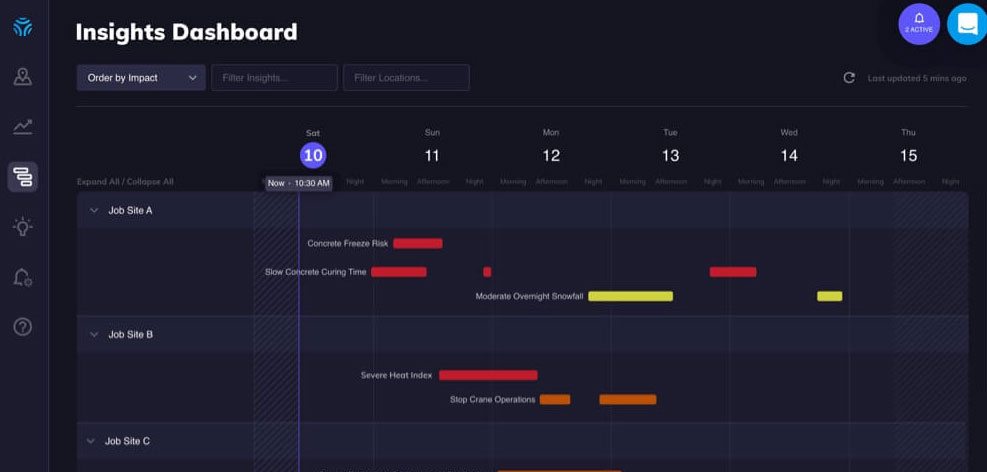
\includegraphics[width=\textwidth]{figs/climacell.jpg}
	\label{f.darksky-calendar}
	\legend{\small Fonte: \cite{dashboard-climacell}.}
\end{figure}

\subsection{Dark Sky}
\label{ss.darksky}
O Dark Sky é uma aplicação para simulação pluviométrica que foi comprada pela Apple em 2020. Uma de suas funcionalidades, apelidada de Time Machine ou “Máquina do Tempo”, em português, consegue simular dados para mais de 15 anos no futuro.

Além disso, o Dark Sky oferece informações meteorológicas hiperlocais, com previsões minuto a minuto para entregar ao usuário informações exatas de quando a chuva vai começar ou acabar.

\begin{figure}[H]
	\caption{\small Função \emph{Time Machine} da aplicação Dark Sky.}
	\centering
	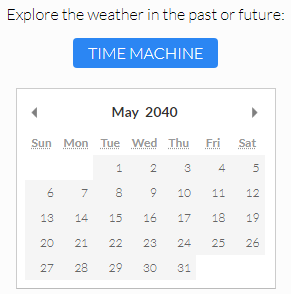
\includegraphics[scale=0.75]{figs/darkskyCalendar.PNG}
	\label{f.darksky-calendar}
	\legend{\small Fonte: \cite{darksky-main}.}
\end{figure}

\subsection{WeatherTAB}
\label{ss.weathertab}
Essa aplicação fornece um serviço de simulação da previsão de tempo há mais de cinquenta anos. Inicialmente o serviço era pago, mas recentemente a empresa decidiu abrir as portas ao público disponibilizando gratuitamente as suas previsões, cobridos por meio de publicidade.

O WeatherTAB fornece previsões meteorológicas com até 18 meses de antecedência, sem perda de precisão, segundo a própria organização ~\cite{weathertab}. Essas previsões são projetadas para ajudar no planejamento de atividades ao ar livre e indicam, com meses de antecedência, as datas em que há pouco ou muito risco de chuva ou neve.

\begin{figure}[H]
	\caption{\small Função de Previsão a Longo Prazo da aplicação WeatherTAB.}
	\centering
	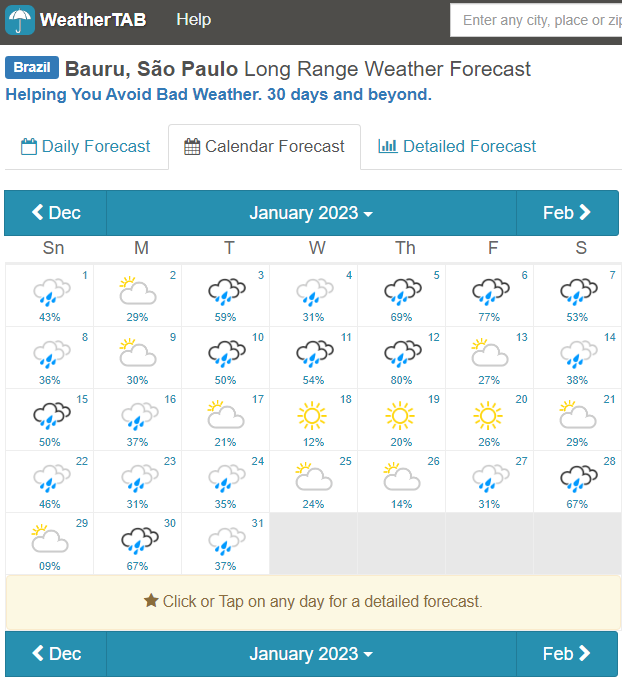
\includegraphics[scale=0.75]{figs/wtab-forecast.png}
	\label{f.darksky-calendar}
	\legend{\small Fonte: \cite{weathertab}.}
\end{figure}
\pagestyle{simple}
\chapter{Projeto do Software}
\label{c.projeto}

O projeto do software é uma solução para a simulação da probabilidade de chuva de um determinado período para uma determinada cidade que tenha disponível dados históricos pluviométricos, de preferência maiores do que 20 anos.

O modelo em questão utiliza a Cadeia de Markov para gerar a probabilidade de ocorrência de chuva, para então determinar se o dia vai ser chuvoso ou seco. Para isso, deve ser analisado previamente um certo intervalo de dias anteriores ao dia a ser previsto. Como dito anteriormente, o trabalho adotou que se a precipitação pluviométrica de certo dia for maior ou igual a 0, então ele é considerado chuvoso. Caso contrário, é considerado seco.

A implementação em MATLAB é possível devido a facilidade de trabalho com vetores e matrizes que a ferramenta proporciona. Dando como \emph{input} as variáveis da tabela, cada uma organizada dentro de um vetor, foi viável a elaboração de um \emph{script} para gerar simular dias chuvosos e secos de um ano inteiro.

A cidade analisada foi Bauru, do estado de São Paulo, que tem disponível dados históricos desde 2002 através da Estacão Automática A705, latitude -22,358052 e longitude -49,028877. O ano simulado foi 2021 para que seja possível realizar uma comparação de resultados no final, a fim de verificar a precisão da simulação realizada neste trabalho.
\section{Especificação}
\label{s.especificacao}

Para realizar a simulação, com base no modelo analisado ~\cite{artigo_modelo}, é necessário efetuar um processo de geração das séries de dias secos e chuvosos através da comparação das probabilidades condicionais \emph{P(C|S)} e \emph{P(C|C)} com um número aleatório \emph{x} entre 0 e 1. O processo é inicializado em qualquer dia do mês simulado, desta forma, a definição do estado inicial (seco ou chuvoso) do dia anterior é obtida a partir de uma fonte meteorológica confiável. Para os demais dias, é feito da seguinte maneira:

\begin{enumerate}
  \item verifica se o dia anterior foi chuvoso ou seco. Nesse trabalho, um dia é considerado chuvoso quando a sua precipitação diária for maior do que 0mm;
  \item se o dia anterior for seco, gera-se um número aleatório \emph{x} entre 0 e 1, e o compara com a probabilidade condicional P(C|S) gerada para o dia atual analisado. Já se o dia anterior foi chuvoso, compara-se o número aleatório \emph{x} com a probabilidade condicional P(C|C) obtida para o dia atual analisado. Essa comparação é feita da seguinte forma:
  \begin{enumerate}[label=(\alph*)]
   \item se x $\leq$ P(C|S) ou P(C|C), o estado do dia atual é considerado chuvoso; 
   \item se x > P(C|S) ou P(C|C), o estado do dia atual é considerado seco.
  \end{enumerate}
\end{enumerate}

As probabilidades condicionais são definidas com base na Cadeia de Markov, com suas fórmulas descritas abaixo:

\[
    P(C|S)=\frac{N(C|S)}{N(C|S)+N(C|S)}=\frac{N(C|S)}{N(S)}
\]
\[
    P(C|C)=\frac{N(C|C)}{N(S|C)+N(C|C)}=\frac{N(C|C)}{N(C)}
\]

\section{Tecnologias Pesquisadas e Escolhidas}
\label{s.tecnologias}

Existem diversas tecnologias que são capazes de realizar a simulação pluviométrica de maneira satisfatória. De todas as analisadas, a ferramenta escolhida foi o MATLAB, uma linguagem de programação de alta performance voltada para o cálculo numérico.

\subsection{MATLAB}
\label{ss.matlab}

Para um projeto que envolve muitos cálculos numéricos e manipulações de extensas matrizes e vetores, o software MATLAB é líder no segmento ~\cite{matlab}. Trata-se de um software robusto que consegue resolver muitos problemas em um tempo muito menor de programação quando comparado a outras linguagens de programação.
A versão escolhida para realizar o trabalho foi a R2021a, lançada em março de 2021, 
porém existem muitas outras versões desde o ano de 1984.
Trata-se de um software proprietário pago, mas existem licenças exclusivas para estudantes de universidade.

\begin{figure}[H]
    \caption{\small Demonstração de sintaxe na IDE do MATLAB.}
	\centering
	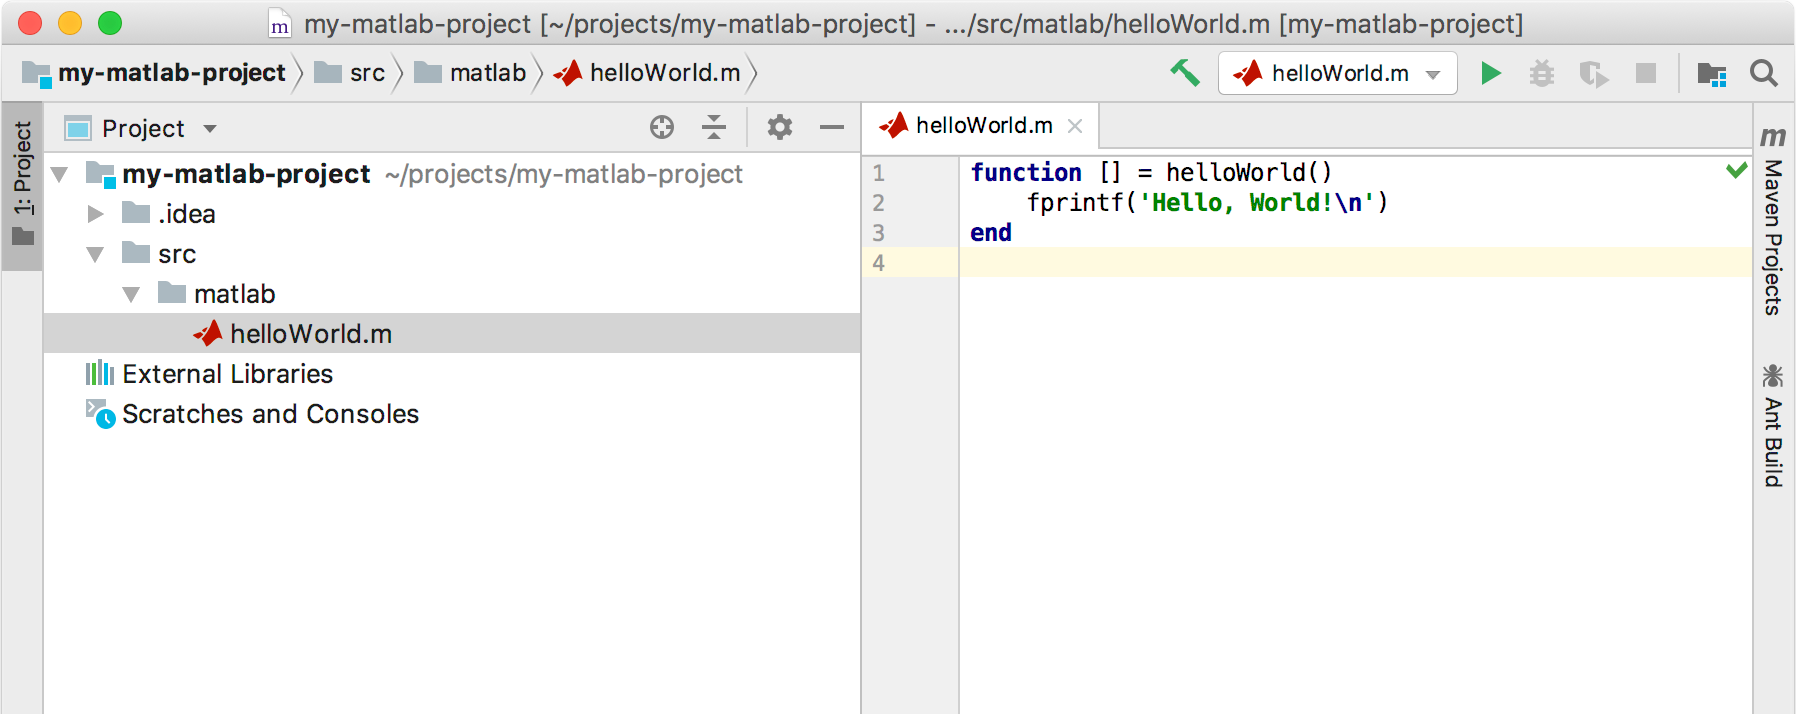
\includegraphics[width=\textwidth]{figs/matlab-syntax.png}
	\label{f.matlab-syntax}
	\legend{\small Fonte: \cite{matlab-jetbrains}.}
\end{figure}

\subsection{Mathematica}
\label{ss.mathematica}

É outro programa que permite resolver problemas matemáticos com certa facilidade, utilizando de várias bibliotecas de programação para auxiliar na resolução de problemas de ciências exatas.
O sistema é utilizado em muitas áreas da computação, como redes neurais, aprendizado de máquina, processamento de imagens, geometria, ciência de dados, visualizações e diversas outras ~\cite{mathematica}.

\begin{figure}[H]
    \caption{\small Demonstração de sintaxe na IDE do Mathematica.}
	\centering
	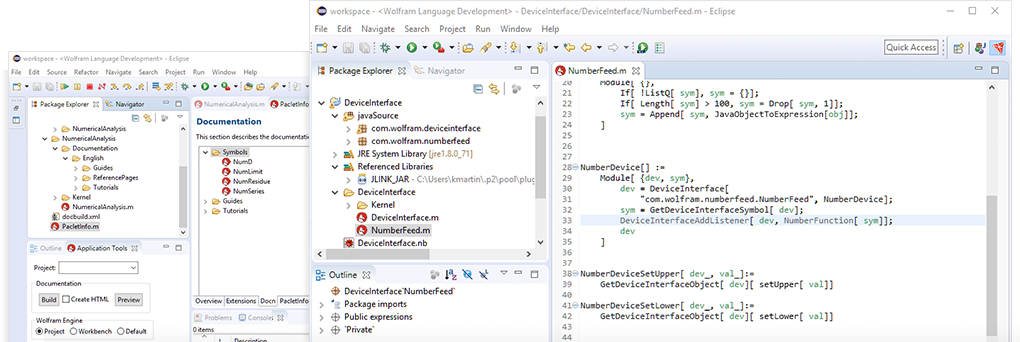
\includegraphics[width=\textwidth]{figs/mathematica-ide.png}
	\label{f.matlab-syntax}
	\legend{\small Fonte: \cite{mathematica}.}
\end{figure}

\subsection{GNU Octave}
\label{ss.gnu}

Em termos de compatibilidade e capacidade computacional, o GNU Octave é considerado a melhor alternativa do MATLAB ~\cite{matlab-alts}. A maioria dos projetos desenvolvidos para o MATLAB também conseguem ser executados no Octave. Além disso, ele roda em qualquer sistema operacional sem nenhuma modificação. 

Ele pode lidar com grandes sintaxes matemáticas e tem ferramentas de plotagem e visualização. Além disso, é um software de código aberto e foi desenvolvido principalmente para cálculos numéricos lineares e não lineares complexos. Ele pode executar trabalhos interativos e em lote e tem compatibilidade com \emph{scripts} MATLAB e outros escritos em Java, C++ ou Fortran.

\begin{figure}[H]
	\caption{\small Demonstração de sintaxe na IDE do GNU Octave.}
	\centering
	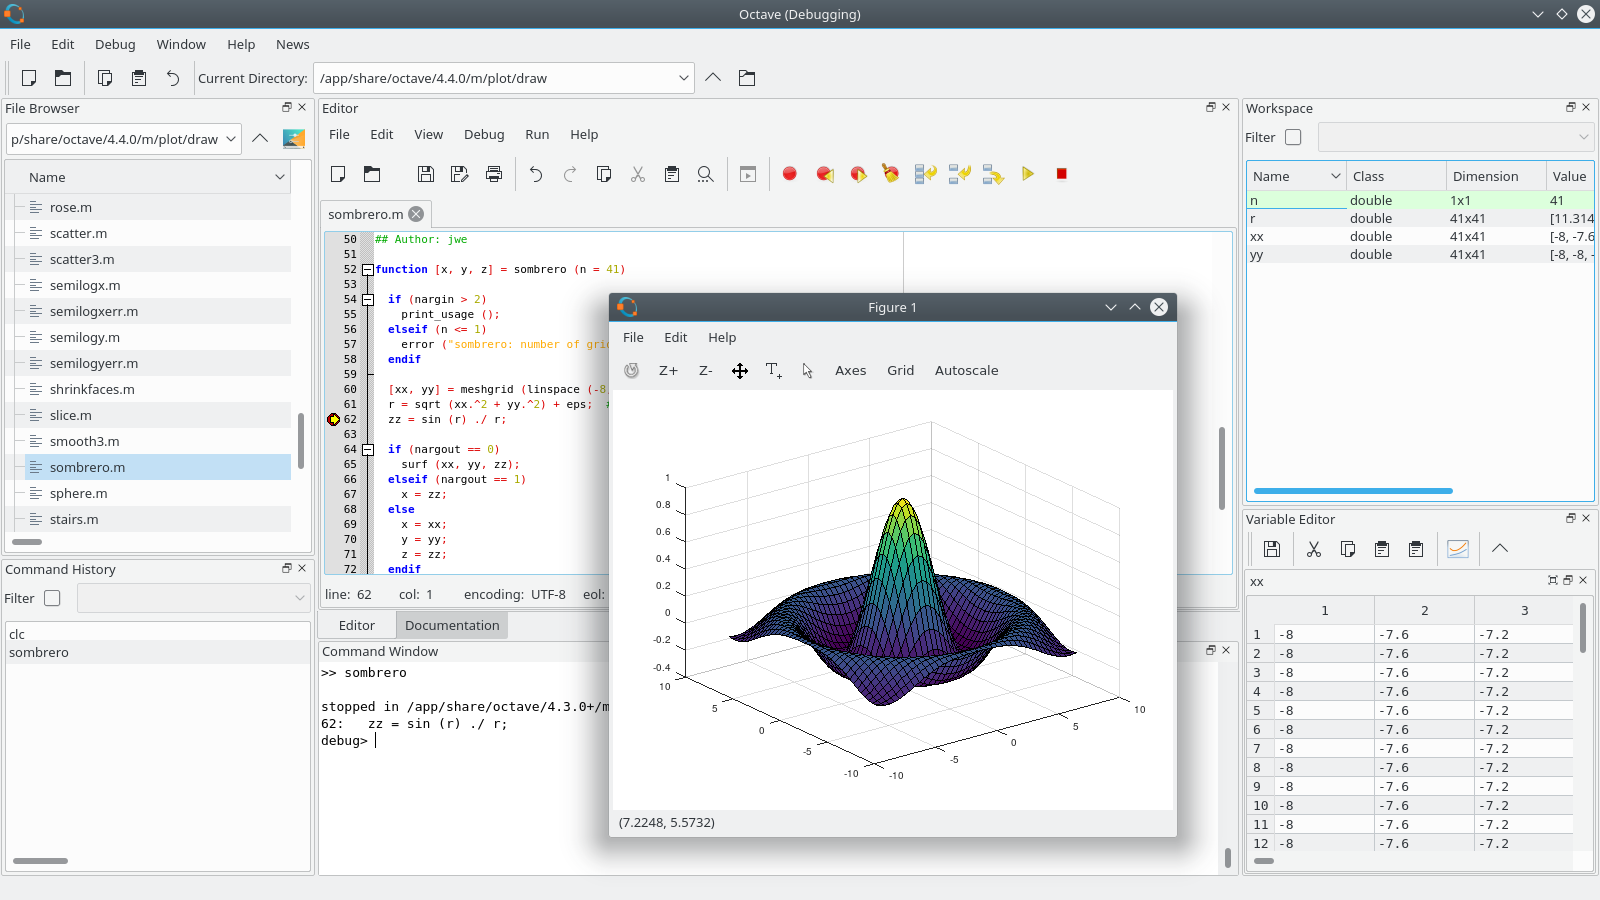
\includegraphics[width=\textwidth]{figs/octave-ide.png}
	\label{f.matlab-syntax}
	\legend{\small Fonte: \cite{octave-ide}.}
\end{figure}
\chapter{Implementação}
\label{c.implementacao}
A implementação foi feita através de um script em Matlab elaborado pelo autor. O script recebe como \emph{input} os dados históricos de todos os dias de um intervalo de anos para uma cidade, e então gera os resultados como \emph{\emph{output}}. A base de dados, inputs, outputs e o script serão tratados com detalhes nos tópicos a seguir.

\section{Base de Dados}
\label{s.basedados}
Para a base de dados, a cidade escolhida foi Bauru, no estado de São Paulo. Bauru tem maiores quantidades de chuva durante o verão, com um inverno mais seco.

Todos os dados obtidos estão disponíveis livre e gratuitamente para consulta no site do Instituto Nacional de Meteorologia (INMET) ~\cite{inmet}. A estacão que mediu os dados tem o código de A705, com local em latitude -22,358052, longitude -49,028877 e altitude de 636,17m. Os dados foram medidos dia a dia, durante todos os meses dos anos de 2002 a 2020, sendo no total 19 anos (6935 dias) de dados. Os dias 29 de fevereiro de cada ano foram desconsiderados por não ter uma quantidade suficiente de dados. 

Os dados disponibilizados são horários, diários ou mensais, de estacões convencionais ou automáticas. Além de dados sobre precipitação, também podem ser consultados dados de temperatura, umidade, vento e pressão atmosférica. As unidades dos dados são:
\begin{itemize}
    \item Temperatura média, máxima, mínima e do ponto de orvalho média (\degree C);
    \item Umidade Relativa do Ar média e mínima (\%);
    \item Precipitação Total (mm);
    \item Velocidade média e rajada máxima do Vento (km/h, m/s);
    \item Pressão atmosférica média (atm).
\end{itemize}


%é

\section{Inputs e Outputs}
\label{s.io}
Para que o script possa funcionar, ele precisa de alguns dados de entrada, chamados de \emph{inputs}. Através desses dados é realizado todo o processamento para então gerar os dados de saída, chamados de \emph{outputs}.
Esses dados devem estar em formatos específicos para atender as necessidades do programa. Caso contrario, o script não funcionará corretamente e acabará em erros.

\subsection{Inputs}
\label{ss.inputs}
Para os dados de entrada, chamados de \emph{inputs}, o script precisa de 12 arquivos em formato .txt que funcionam como matrizes, cada um representando cada mês, de janeiro a dezembro. Cada um desses arquivos deve ter 31 linhas, representando os dias, e no mínimo 2 colunas, representando a base histórica dos anos. Além desses 12 arquivos, um arquivo extra é necessário com a precipitação diária do dia anterior ao dia mais antigo da base de dados, pois a Cadeia de Markov a qual o modelo se baseia utiliza dados dos dias anteriores para gerar as probabilidades condicionais necessárias. Dentro desses arquivos devem estar dados da precipitação diária em milímetros, separados por espaços e com casas decimais delimitadas por um ponto em vez de vírgula, provenientes diretamente da base de dados escolhida. 

O quadro \ref{q.input} demonstra um exemplo de um arquivo .txt que pode ser utilizado como \emph{input}. Percebe-se que o quadro tem 31 linhas, que representam os dias, e 3 colunas, que representam uma base histórica de três anos para um determinado mês. Assim, se a coluna 2 representar o ano de 2019, a terceira linha será o dia 3 de janeiro, portanto o script tem a informação de que a precipitação diária do dia 3 de janeiro de 2019 foi 1,4mm.

Para dados reais, quanto maior o número de colunas, melhor será a simulação pluviométrica. Isso acontece porque as colunas representam os anos, e a Cadeia de Markov tem um grau de precisão maior conforme o número de dados históricos é aumentado.

\begin{table}[H]
\caption{Exemplo de \emph{input} utilizado pelo script para o processamento da simulação.}
\label{q.input}
\centering

\begin{tabular}{|c|c|c|}
\hline
0.2 & 0   & 0.4  \\ \hline
0   & 0   & 0    \\ \hline
17  & 1.4 & 0    \\ \hline
0   & 0   & 2    \\ \hline
0   & 6.8 & 2    \\ \hline
0   & 0   & 0    \\ \hline
0   & 0   & 0    \\ \hline
0   & 9   & 0    \\ \hline
5   & 12  & 16.8 \\ \hline
0   & 10  & 0    \\ \hline
0   & 0   & 0    \\ \hline
0   & 0   & 0    \\ \hline
6   & 0   & 0    \\ \hline
0.8 & 0   & 0    \\ \hline
2   & 0   & 0    \\ \hline
0   & 0   & 0    \\ \hline
0   & 0   & 0    \\ \hline
0   & 9   & 0    \\ \hline
0   & 4   & 0    \\ \hline
0   & 0   & 34   \\ \hline
1.6 & 0   & 0    \\ \hline
0   & 0   & 0    \\ \hline
0   & 0   & 5    \\ \hline
0   & 0   & 0    \\ \hline
0   & 6   & 0    \\ \hline
0   & 0   & 4    \\ \hline
9   & 0   & 16   \\ \hline
0   & 0   & 0    \\ \hline
0   & 5   & 0    \\ \hline
0   & 0   & 0    \\ \hline
3.8 & 0   & 23   \\ \hline
\end{tabular}
\vspace*{15px}
\legend{\small Fonte: Elaborado pelo autor.}
\end{table}

\subsection{Outputs}
\label{ss.outputs}
Depois de processados os dados de entrada, o script gera automaticamente, em milésimos de segundos, o resultado bruto da simulação com base no modelo estudado.

São dois os resultados gerados, também em formato .txt representando matrizes. O primeiro deles é uma matriz com 31 linhas e 12 colunas, ou seja, um ano inteiro simulado, com probabilidades de chuva entre 0 e 1 separadas por um espaço simples, conforme demonstrado no quadro \ref{q.output1}. O segundo output, e o mais importante, também é uma matriz com 31 linhas e 12 colunas, mas com dados binários (0 ou 1) representando se os dias vão ser secos ou chuvosos, respectivamente. O quadro \ref{q.output2} demonstra um exemplo do segundo resultado gerado pelo script.

\begin{table}[H]
\caption{Exemplo de output com probabilidades condicionais gerado pelo script.}
\label{q.output1}
\centering
\begin{tabular}{|c|c|c|c|c|c|c|c|c|c|c|c|}
\hline
0,26 & 0,61 & 0,90 & 0,02 & 0,33 & 0,23 & 0,63 & 0,03 & 0,50 & 0,25 & 0,49 & 0,23 \\ \hline
0,65 & 0,23 & 0,07 & 0,63 & 0,57 & 0,30 & 0,88 & 0,73 & 0,89 & 0,61 & 0,30 & 0,06 \\ \hline
0,35 & 0,09 & 0,32 & 0,92 & 0,11 & 0,82 & 0,10 & 0,88 & 0,84 & 0,56 & 0,67 & 0,84 \\ \hline
0,65 & 0,77 & 0,02 & 0,90 & 0,84 & 0,52 & 0,56 & 0,07 & 0,26 & 0,03 & 0,87 & 0,59 \\ \hline
0,66 & 0,55 & 0,35 & 0,56 & 0,76 & 0,65 & 0,67 & 0,64 & 0,06 & 0,31 & 0,92 & 0,99 \\ \hline
0,53 & 0,73 & 0,83 & 0,60 & 0,03 & 0,89 & 0,76 & 0,15 & 0,99 & 0,20 & 0,40 & 0,34 \\ \hline
0,74 & 0,20 & 0,84 & 0,99 & 0,95 & 0,56 & 0,40 & 1,00 & 0,73 & 0,99 & 0,96 & 0,12 \\ \hline
0,14 & 0,83 & 0,46 & 0,95 & 0,44 & 0,86 & 0,66 & 0,76 & 0,63 & 0,98 & 0,00 & 0,51 \\ \hline
0,61 & 0,48 & 0,35 & 0,76 & 0,09 & 0,44 & 0,10 & 0,34 & 0,28 & 0,61 & 0,19 & 0,24 \\ \hline
0,22 & 0,76 & 0,87 & 0,29 & 0,97 & 0,06 & 0,26 & 0,32 & 0,24 & 0,85 & 0,14 & 0,54 \\ \hline
0,87 & 0,96 & 0,36 & 0,79 & 0,22 & 0,99 & 0,25 & 0,68 & 0,84 & 0,17 & 0,85 & 0,48 \\ \hline
0,30 & 0,05 & 0,36 & 0,11 & 0,20 & 0,73 & 0,61 & 0,80 & 0,56 & 0,67 & 0,83 & 0,46 \\ \hline
0,18 & 0,74 & 0,28 & 0,35 & 0,06 & 0,25 & 0,16 & 0,72 & 0,98 & 0,91 & 0,88 & 0,77 \\ \hline
0,01 & 0,70 & 0,73 & 0,63 & 0,22 & 0,08 & 0,97 & 0,53 & 0,62 & 0,79 & 0,96 & 0,10 \\ \hline
0,35 & 0,50 & 0,28 & 0,69 & 0,72 & 0,43 & 0,71 & 0,46 & 0,79 & 0,71 & 0,92 & 0,66 \\ \hline
0,92 & 0,92 & 0,92 & 0,25 & 0,27 & 0,59 & 0,64 & 0,11 & 0,22 & 0,23 & 0,34 & 0,76 \\ \hline
0,36 & 0,54 & 0,36 & 0,39 & 0,68 & 0,69 & 0,81 & 0,04 & 0,49 & 0,70 & 0,22 & 1,00 \\ \hline
0,63 & 0,82 & 0,03 & 0,20 & 0,83 & 0,74 & 0,15 & 0,83 & 0,85 & 0,49 & 0,17 & 0,16 \\ \hline
0,10 & 0,21 & 0,06 & 0,99 & 0,46 & 0,91 & 0,48 & 0,65 & 0,60 & 0,13 & 0,06 & 0,84 \\ \hline
0,42 & 1,00 & 0,74 & 0,42 & 0,78 & 0,96 & 0,27 & 0,72 & 0,94 & 0,44 & 0,84 & 0,48 \\ \hline
0,22 & 0,32 & 0,48 & 0,86 & 0,12 & 0,51 & 0,78 & 0,97 & 0,25 & 0,76 & 0,16 & 0,11 \\ \hline
0,34 & 0,89 & 0,06 & 0,70 & 0,52 & 0,62 & 0,11 & 0,11 & 0,15 & 0,31 & 0,41 & 0,40 \\ \hline
0,44 & 0,96 & 0,66 & 0,18 & 0,90 & 0,12 & 0,23 & 0,82 & 0,21 & 0,05 & 0,23 & 0,40 \\ \hline
0,71 & 0,16 & 0,62 & 0,02 & 0,95 & 0,07 & 0,87 & 0,97 & 0,73 & 0,72 & 0,16 & 0,38 \\ \hline
0,86 & 0,89 & 0,49 & 0,85 & 0,00 & 0,90 & 0,93 & 0,32 & 0,62 & 0,80 & 0,11 & 0,66 \\ \hline
0,01 & 0,51 & 0,59 & 0,84 & 0,75 & 0,37 & 0,67 & 0,99 & 0,34 & 0,14 & 0,95 & 0,56 \\ \hline
0,34 & 0,35 & 0,40 & 0,29 & 0,53 & 0,22 & 0,17 & 0,04 & 0,10 & 0,13 & 0,20 & 0,46 \\ \hline
0,62 & 0,62 & 0,69 & 0,02 & 0,15 & 0,87 & 0,54 & 0,49 & 0,28 & 0,08 & 0,61 & 0,06 \\ \hline
0,69 & -    & 0,93 & 0,84 & 0,08 & 0,19 & 0,45 & 0,01 & 0,43 & 0,62 & 0,61 & 0,02 \\ \hline
0,24 & -    & 0,50 & 0,09 & 0,76 & 0,59 & 0,77 & 0,80 & 0,09 & 0,40 & 0,16 & 0,46 \\ \hline
0,47 & -    & 0,72 & -    & 0,51 & -    & 0,33 & 0,30 & -    & 0,60 & -    & 0,91 \\ \hline
\end{tabular}
\vspace*{15px}
\legend{\small Fonte: Elaborado pelo autor.}
\end{table}

\begin{table}[H]
\caption{Exemplo de output com dados binários gerado pelo script.}
\label{q.output2}
\centering
\begin{tabular}{|c|c|c|c|c|c|c|c|c|c|c|c|}
\hline
1 & 1 & 0 & 1 & 1 & 0 & 0 & 1 & 0 & 1 & 0 & 0 \\ \hline
0 & 1 & 1 & 1 & 0 & 1 & 1 & 0 & 1 & 1 & 0 & 0 \\ \hline
0 & 1 & 1 & 1 & 1 & 1 & 0 & 1 & 0 & 1 & 1 & 0 \\ \hline
0 & 1 & 1 & 1 & 1 & 1 & 1 & 1 & 1 & 1 & 1 & 1 \\ \hline
0 & 1 & 1 & 0 & 0 & 1 & 0 & 1 & 1 & 1 & 1 & 1 \\ \hline
0 & 1 & 0 & 1 & 0 & 0 & 0 & 1 & 0 & 1 & 1 & 1 \\ \hline
1 & 1 & 1 & 1 & 0 & 1 & 1 & 1 & 0 & 0 & 1 & 0 \\ \hline
1 & 0 & 1 & 1 & 1 & 1 & 0 & 0 & 1 & 0 & 1 & 0 \\ \hline
1 & 0 & 1 & 0 & 1 & 1 & 1 & 1 & 0 & 0 & 0 & 1 \\ \hline
0 & 1 & 0 & 1 & 0 & 0 & 1 & 1 & 0 & 0 & 1 & 0 \\ \hline
0 & 0 & 0 & 0 & 1 & 0 & 1 & 1 & 1 & 0 & 0 & 1 \\ \hline
1 & 1 & 0 & 0 & 1 & 0 & 0 & 0 & 1 & 1 & 1 & 0 \\ \hline
1 & 0 & 0 & 1 & 1 & 0 & 1 & 1 & 1 & 0 & 0 & 1 \\ \hline
0 & 0 & 1 & 0 & 0 & 1 & 1 & 1 & 1 & 0 & 0 & 0 \\ \hline
0 & 1 & 0 & 0 & 1 & 1 & 0 & 0 & 0 & 1 & 1 & 1 \\ \hline
0 & 1 & 0 & 0 & 0 & 1 & 0 & 1 & 1 & 1 & 1 & 0 \\ \hline
0 & 1 & 0 & 0 & 0 & 0 & 0 & 1 & 0 & 0 & 0 & 0 \\ \hline
1 & 1 & 0 & 1 & 1 & 1 & 1 & 0 & 0 & 0 & 0 & 0 \\ \hline
0 & 0 & 1 & 0 & 0 & 1 & 0 & 1 & 0 & 0 & 1 & 1 \\ \hline
1 & 0 & 1 & 0 & 0 & 1 & 1 & 0 & 1 & 1 & 1 & 1 \\ \hline
0 & 0 & 1 & 1 & 1 & 1 & 1 & 0 & 0 & 0 & 1 & 1 \\ \hline
1 & 0 & 1 & 0 & 1 & 0 & 0 & 1 & 0 & 0 & 1 & 1 \\ \hline
1 & 0 & 0 & 1 & 1 & 1 & 1 & 1 & 0 & 0 & 0 & 1 \\ \hline
0 & 0 & 1 & 1 & 0 & 1 & 0 & 1 & 1 & 1 & 0 & 1 \\ \hline
0 & 0 & 1 & 0 & 0 & 0 & 1 & 1 & 1 & 0 & 1 & 1 \\ \hline
0 & 1 & 1 & 0 & 1 & 0 & 0 & 1 & 1 & 1 & 1 & 0 \\ \hline
0 & 1 & 1 & 1 & 0 & 1 & 1 & 0 & 0 & 0 & 0 & 1 \\ \hline
1 & 1 & 1 & 1 & 0 & 0 & 1 & 1 & 1 & 0 & 0 & 0 \\ \hline
0 & - & 1 & 0 & 0 & 1 & 0 & 0 & 1 & 1 & 0 & 1 \\ \hline
0 & - & 1 & 1 & 1 & 1 & 1 & 0 & 0 & 0 & 1 & 1 \\ \hline
1 & - & 0 & - & 1 & - & 1 & 0 & - & 1 & - & 0 \\ \hline
\end{tabular}
\vspace*{15px}
\legend{\small Fonte: Elaborado pelo autor.}
\end{table}



\section{Script}
\label{s.io}
O script foi programado no ambiente de desenvolvimento do Matlab, então tem o formato .m padrão da linguagem. São 251 linhas de código comentadas e elaboradas de maneira eficiente para que o tempo de processamento seja o mais rápido possível.

O autor deixou disponível de maneira integral e aberta o script, bem como a base de dados e os resultados brutos da simulação em sua página do GitHub \cite{script-tcc} para que quaisquer interessados possam consultar ou até mesmo utilizar para algum projeto pessoal. Na figura \ref{f.example-script} é possível observar parte de uma função do script.

\begin{figure}[H]
	\caption{\small Parte de uma função do script.}
	\centering
	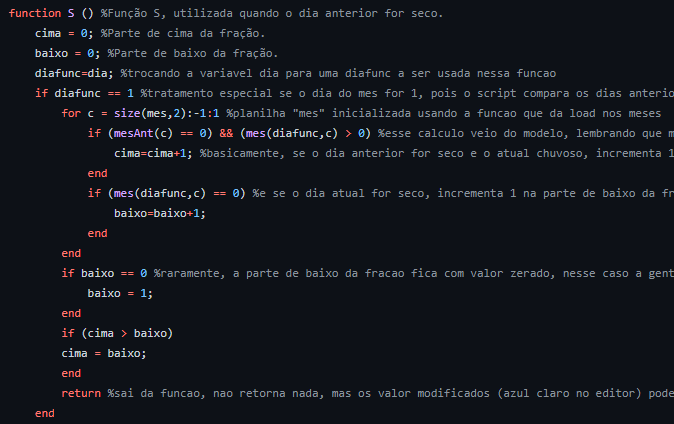
\includegraphics[width=\textwidth]{figs/example-script.png}
	\label{f.example-script}
	\legend{\small Fonte: Elaborado pelo Autor.}
\end{figure}







%é
\chapter{Resultados}
\label{c.resultados}
Ao executar o script, a simulação foi salva em dois arquivos de texto. O primeiro, representado no quadro \ref{q.res1}, demonstra a probabilidade de chuva para todos os 365 dias do ano de 2021. O segundo arquivo, representado no quadro \ref{q.res2}, e também foco principal do trabalho, mostra se os dias vão ser chuvosos ou não. Para isso, utiliza o numero 1 e 0 se forem chuvosos ou secos, respectivamente. As colunas representam os meses, de janeiro a dezembro, com um total de 12 colunas. De forma similar, as linhas representam os dias, de 1 a 31, com um total de 31 linhas.

\begin{table}[H]
\caption{Resultado da simulação com as probabilidades condicionais geradas pelo script.}
\label{q.res1}
\centering
\begin{tabular}{|c|c|c|c|c|c|c|c|c|c|c|c|}
\hline
0.5  & 0.07 & 0.08 & 0    & 0    & 0.08 & 0.13 & 0.06 & 0.42 & 0.5  & 0.2  & 0.64 \\ \hline
0.67 & 0.15 & 0.23 & 0.19 & 0.13 & 0.25 & 0.13 & 0.06 & 0    & 0.5  & 0.23 & 0.08 \\ \hline
0.9  & 0.56 & 0.17 & 0.75 & 0.5  & 0.71 & 0.06 & 0.13 & 0.06 & 0.6  & 0.08 & 0.33 \\ \hline
0.64 & 0.1  & 0.18 & 0.6  & 0.19 & 0.25 & 0.13 & 0.06 & 0.13 & 0.5  & 0.36 & 0.25 \\ \hline
0.7  & 0.08 & 0.08 & 0.5  & 0.23 & 0.4  & 0    & 0.06 & 0.06 & 1    & 0.08 & 0.36 \\ \hline
0.25 & 0.33 & 0.27 & 0.57 & 0    & 0.75 & 0.06 & 0.06 & 0.06 & 0.25 & 0.25 & 0.36 \\ \hline
1    & 0.56 & 0.17 & 0.23 & 0    & 0.6  & 0.06 & 0.12 & 0.13 & 0.2  & 0.5  & 0.6  \\ \hline
1    & 0.75 & 0.25 & 0.07 & 0.29 & 0.07 & 0.13 & 0.06 & 0.06 & 0.17 & 0.5  & 0.8  \\ \hline
0.5  & 0.75 & 0.14 & 0.14 & 0.25 & 0    & 0.06 & 0    & 0.06 & 0.5  & 0.4  & 0.33 \\ \hline
0.11 & 0.56 & 0.21 & 0.2  & 0.06 & 0.38 & 0.33 & 0    & 1    & 0.08 & 0.36 & 0.63 \\ \hline
0.44 & 0.22 & 0.45 & 0.67 & 0.06 & 0.13 & 0.36 & 0    & 0.33 & 0.06 & 0    & 0.3  \\ \hline
1    & 0.11 & 0.17 & 0.06 & 0.13 & 0.06 & 0.13 & 0    & 0    & 0.21 & 0.13 & 0.63 \\ \hline
0.75 & 0.5  & 0    & 0.36 & 0    & 0.13 & 0.12 & 0    & 0    & 0.6  & 0.36 & 0.18 \\ \hline
0.89 & 0.8  & 0.45 & 0.23 & 0.2  & 0.13 & 0.06 & 0.12 & 0.06 & 0.17 & 0.78 & 0.27 \\ \hline
0.55 & 0.7  & 0.6  & 0.14 & 0.15 & 0.06 & 0    & 0    & 0    & 0.18 & 0.8  & 0.89 \\ \hline
0.67 & 0.73 & 0.17 & 0.21 & 0.25 & 0.31 & 0.12 & 0.12 & 0.19 & 0.15 & 0.5  & 0.71 \\ \hline
0.77 & 0.9  & 0.07 & 0.06 & 0.07 & 0    & 0.06 & 0.06 & 0.06 & 0.14 & 0    & 0.63 \\ \hline
0.9  & 0.38 & 0.23 & 0    & 0.2  & 0    & 0.2  & 0.06 & 0.06 & 0.29 & 0.31 & 0.07 \\ \hline
0.78 & 0.5  & 0.2  & 0.06 & 0.38 & 0.12 & 0.07 & 0.06 & 0.19 & 0.31 & 0.25 & 0.5  \\ \hline
0.75 & 1    & 0.42 & 0.13 & 1    & 0.13 & 0.06 & 0.13 & 0.36 & 0.4  & 0.15 & 0.44 \\ \hline
0.8  & 0.55 & 0.5  & 0.31 & 0.75 & 0    & 0.06 & 0.07 & 0.08 & 0.27 & 0.13 & 0.67 \\ \hline
0.56 & 0.8  & 0.44 & 0.23 & 0.23 & 0.14 & 0.2  & 0    & 0.2  & 0.38 & 0.42 & 0.45 \\ \hline
0.75 & 0.75 & 0.17 & 0.67 & 0.33 & 0    & 0.06 & 0.06 & 0.06 & 0.17 & 1    & 0.88 \\ \hline
0.3  & 0.36 & 0.15 & 0.2  & 0.17 & 0.06 & 0    & 0    & 0.19 & 0.14 & 0.2  & 0.58 \\ \hline
0.4  & 0.83 & 0.5  & 0.5  & 0.25 & 0.13 & 0.2  & 0.27 & 0.27 & 0.13 & 0.23 & 0.2  \\ \hline
0.57 & 0.86 & 0.33 & 0.13 & 0.75 & 0.4  & 0    & 0    & 0.25 & 0.45 & 0.36 & 0.44 \\ \hline
0.67 & 0.6  & 0.14 & 0.13 & 0.33 & 0    & 0    & 0.36 & 0    & 0.17 & 0.25 & 0.09 \\ \hline
0.85 & 0.67 & 0.13 & 0.13 & 0.4  & 0    & 0    & 0    & 0.07 & 0.56 & 0.14 & 0.25 \\ \hline
0.92 & -    & 0.06 & 0.12 & 0.43 & 0.06 & 0.06 & 0    & 0.06 & 0.06 & 0.33 & 0.29 \\ \hline
1    & -    & 0.29 & 0.29 & 0    & 0.06 & 0    & 0.06 & 0.2  & 0.64 & 0.06 & 0.18 \\ \hline
0.56 & -    & 0    & -    & 0.33 & -    & 0.06 & 0.12 & -    & 0.83 & -    & 0.8  \\ \hline
\end{tabular}
\vspace*{15px}
\legend{\small Fonte: Elaborado pelo autor.}
\end{table}


\begin{table}[H]
\caption{Resultado principal da simulação com os dados binários gerados pelo script.}
\label{q.res2}
\centering
\begin{tabular}{|c|c|c|c|c|c|c|c|c|c|c|c|}
\hline
1 & 0 & 0 & 0 & 0 & 0 & 0 & 0 & 0 & 1 & 0 & 0 \\ \hline
1 & 1 & 0 & 1 & 1 & 1 & 0 & 0 & 0 & 1 & 0 & 0 \\ \hline
1 & 0 & 0 & 1 & 0 & 0 & 0 & 0 & 0 & 1 & 0 & 0 \\ \hline
1 & 0 & 0 & 1 & 0 & 0 & 0 & 0 & 0 & 1 & 0 & 0 \\ \hline
0 & 0 & 0 & 1 & 0 & 1 & 0 & 0 & 0 & 1 & 0 & 0 \\ \hline
0 & 1 & 0 & 0 & 0 & 1 & 0 & 0 & 0 & 0 & 1 & 1 \\ \hline
1 & 1 & 0 & 0 & 0 & 0 & 0 & 0 & 0 & 1 & 1 & 1 \\ \hline
1 & 1 & 0 & 0 & 1 & 0 & 0 & 0 & 0 & 1 & 1 & 0 \\ \hline
0 & 1 & 0 & 0 & 0 & 0 & 1 & 0 & 1 & 0 & 0 & 1 \\ \hline
0 & 0 & 0 & 1 & 0 & 0 & 0 & 0 & 1 & 0 & 0 & 0 \\ \hline
0 & 0 & 0 & 0 & 0 & 0 & 0 & 0 & 0 & 0 & 0 & 1 \\ \hline
1 & 1 & 0 & 0 & 0 & 0 & 0 & 0 & 0 & 0 & 0 & 0 \\ \hline
1 & 1 & 0 & 0 & 0 & 0 & 0 & 0 & 0 & 0 & 1 & 0 \\ \hline
1 & 1 & 1 & 0 & 0 & 0 & 0 & 0 & 0 & 0 & 1 & 1 \\ \hline
0 & 1 & 0 & 0 & 1 & 0 & 0 & 0 & 0 & 0 & 1 & 1 \\ \hline
1 & 1 & 0 & 0 & 0 & 0 & 0 & 0 & 0 & 0 & 1 & 1 \\ \hline
1 & 0 & 0 & 0 & 0 & 0 & 0 & 0 & 0 & 0 & 0 & 0 \\ \hline
1 & 0 & 0 & 0 & 1 & 0 & 0 & 0 & 0 & 0 & 0 & 0 \\ \hline
1 & 1 & 0 & 0 & 1 & 0 & 0 & 0 & 0 & 1 & 0 & 1 \\ \hline
1 & 1 & 1 & 0 & 1 & 0 & 0 & 0 & 0 & 0 & 0 & 1 \\ \hline
1 & 1 & 0 & 0 & 0 & 0 & 0 & 0 & 0 & 1 & 0 & 1 \\ \hline
1 & 1 & 0 & 1 & 0 & 0 & 0 & 0 & 0 & 0 & 1 & 1 \\ \hline
0 & 0 & 0 & 0 & 0 & 0 & 0 & 0 & 0 & 0 & 1 & 1 \\ \hline
0 & 0 & 1 & 1 & 0 & 0 & 0 & 0 & 0 & 0 & 0 & 0 \\ \hline
0 & 1 & 1 & 0 & 1 & 1 & 0 & 0 & 0 & 0 & 0 & 0 \\ \hline
1 & 1 & 0 & 0 & 1 & 0 & 0 & 0 & 0 & 0 & 0 & 0 \\ \hline
1 & 1 & 0 & 0 & 1 & 0 & 0 & 0 & 0 & 0 & 0 & 0 \\ \hline
1 & 0 & 0 & 0 & 1 & 0 & 0 & 0 & 0 & 0 & 0 & 1 \\ \hline
1 & - & 0 & 0 & 0 & 0 & 0 & 0 & 0 & 0 & 0 & 0 \\ \hline
1 & - & 0 & 0 & 0 & 0 & 0 & 0 & 1 & 1 & 0 & 1 \\ \hline
0 & - & 0 & - & 0 & - & 0 & 0 & - & 0 & - & 1 \\ \hline
\end{tabular}
\vspace*{15px}
\legend{\small Fonte: Elaborado pelo autor.}
\end{table}

\section{Análise mês a mês}

\subsection{Janeiro}
\begin{figure}[H]
	\caption{\small Chuva x Dia - Janeiro/2021}
	\centering
	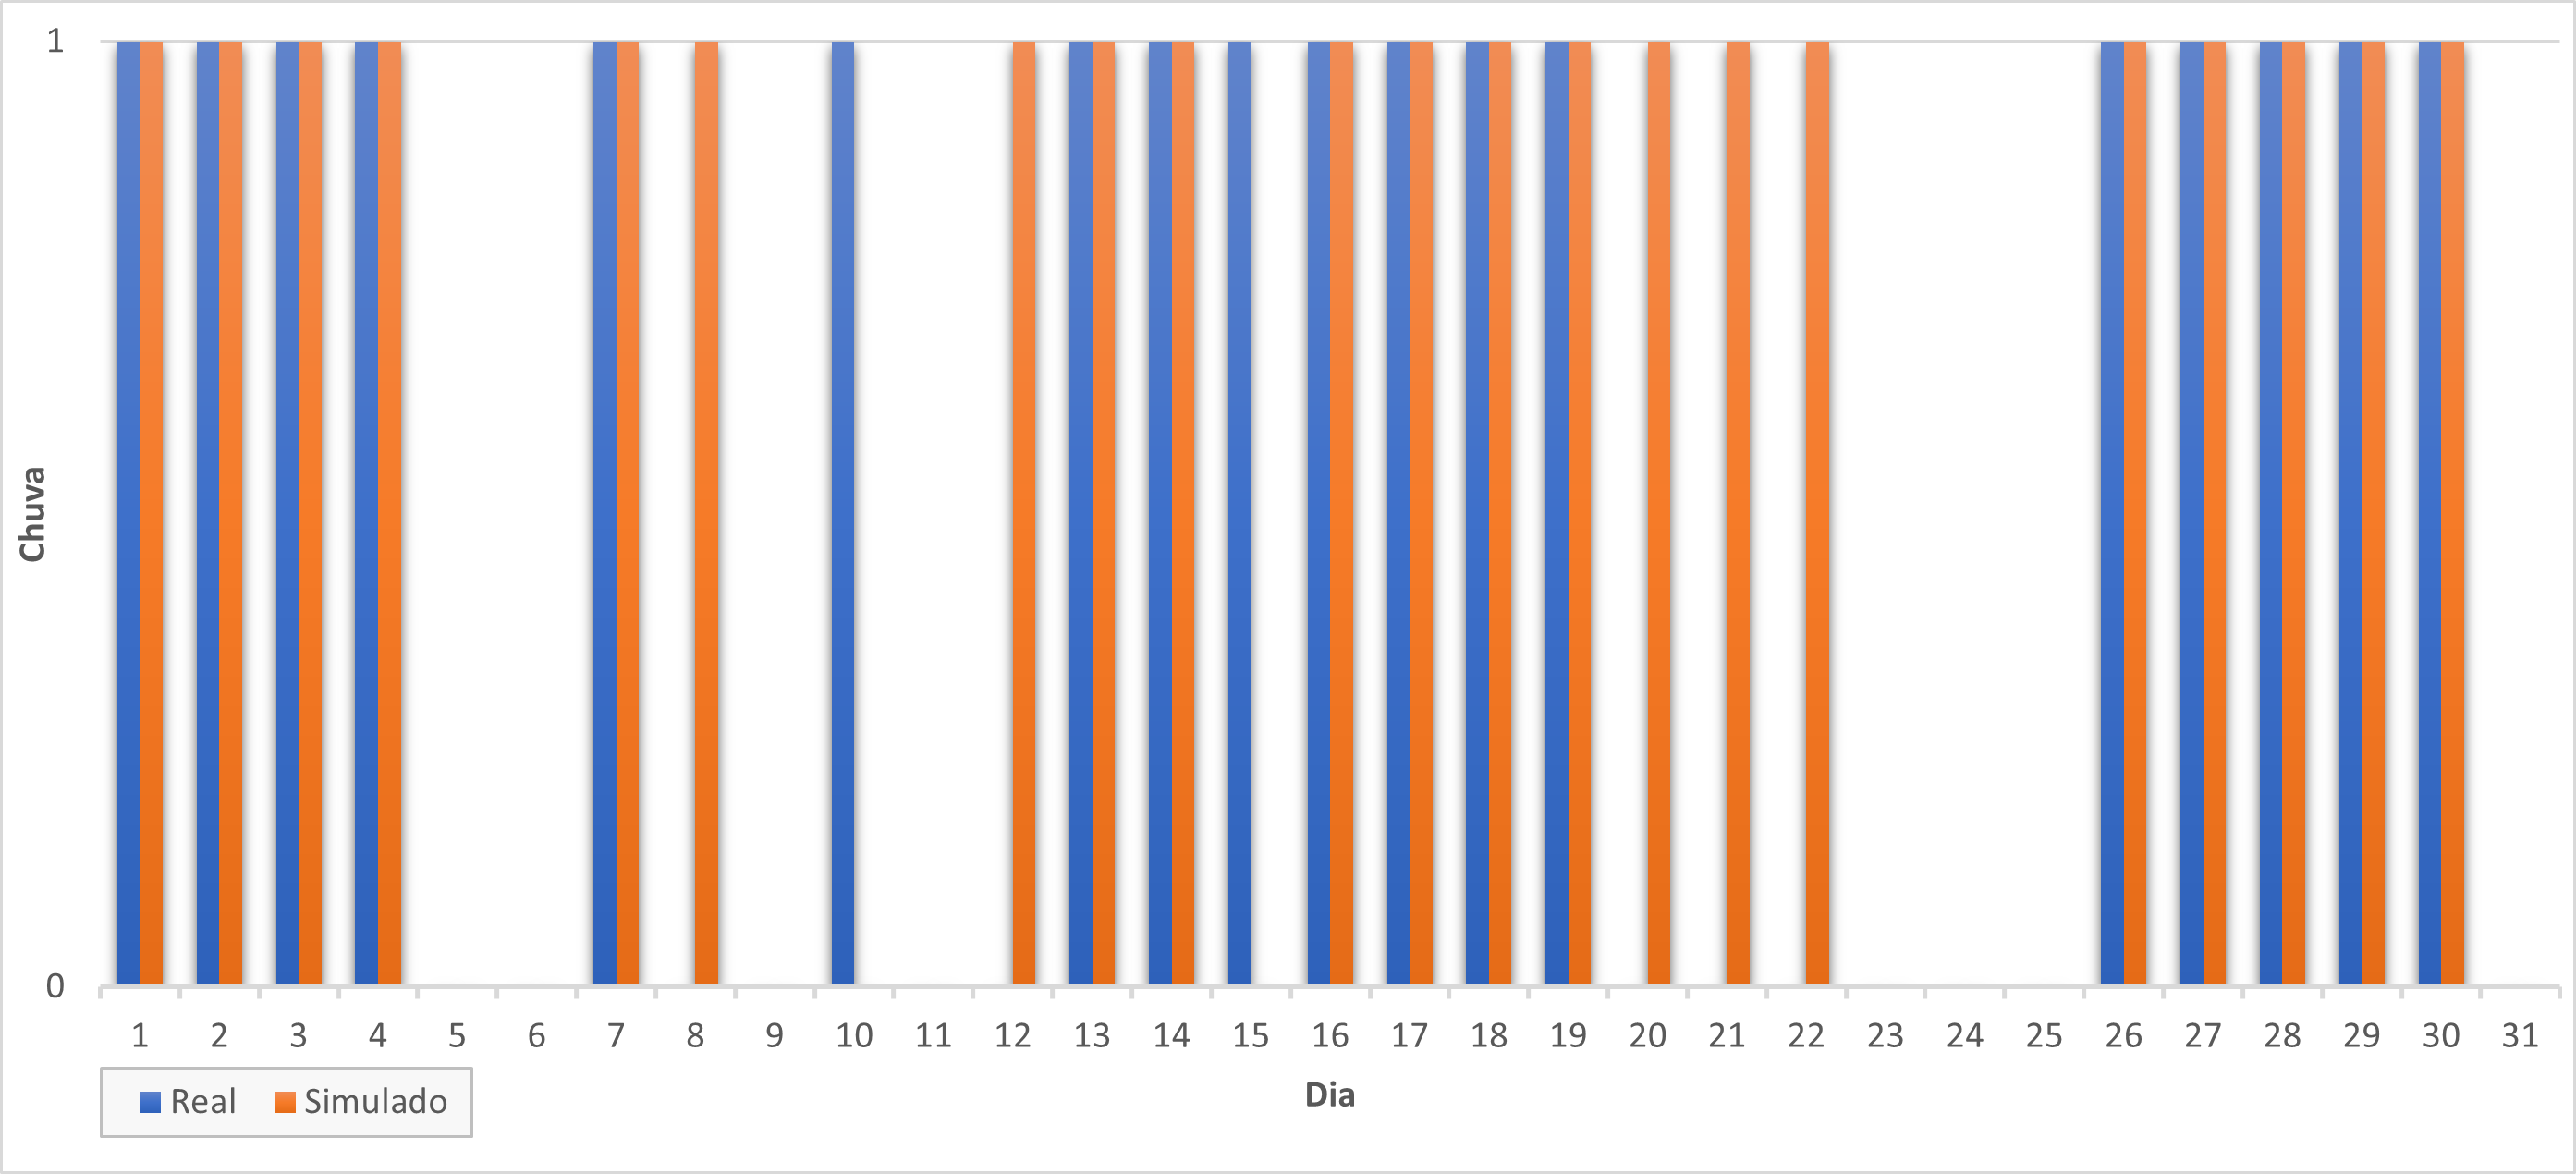
\includegraphics[width=\textwidth]{figs/jan.png}
	\label{f.rjan}
	\legend{\small Fonte: Elaborado pelo autor.}
\end{figure}

\subsection{Fevereiro}
\begin{figure}[H]
	\caption{\small Chuva x Dia - Fevereiro/2021}
	\centering
	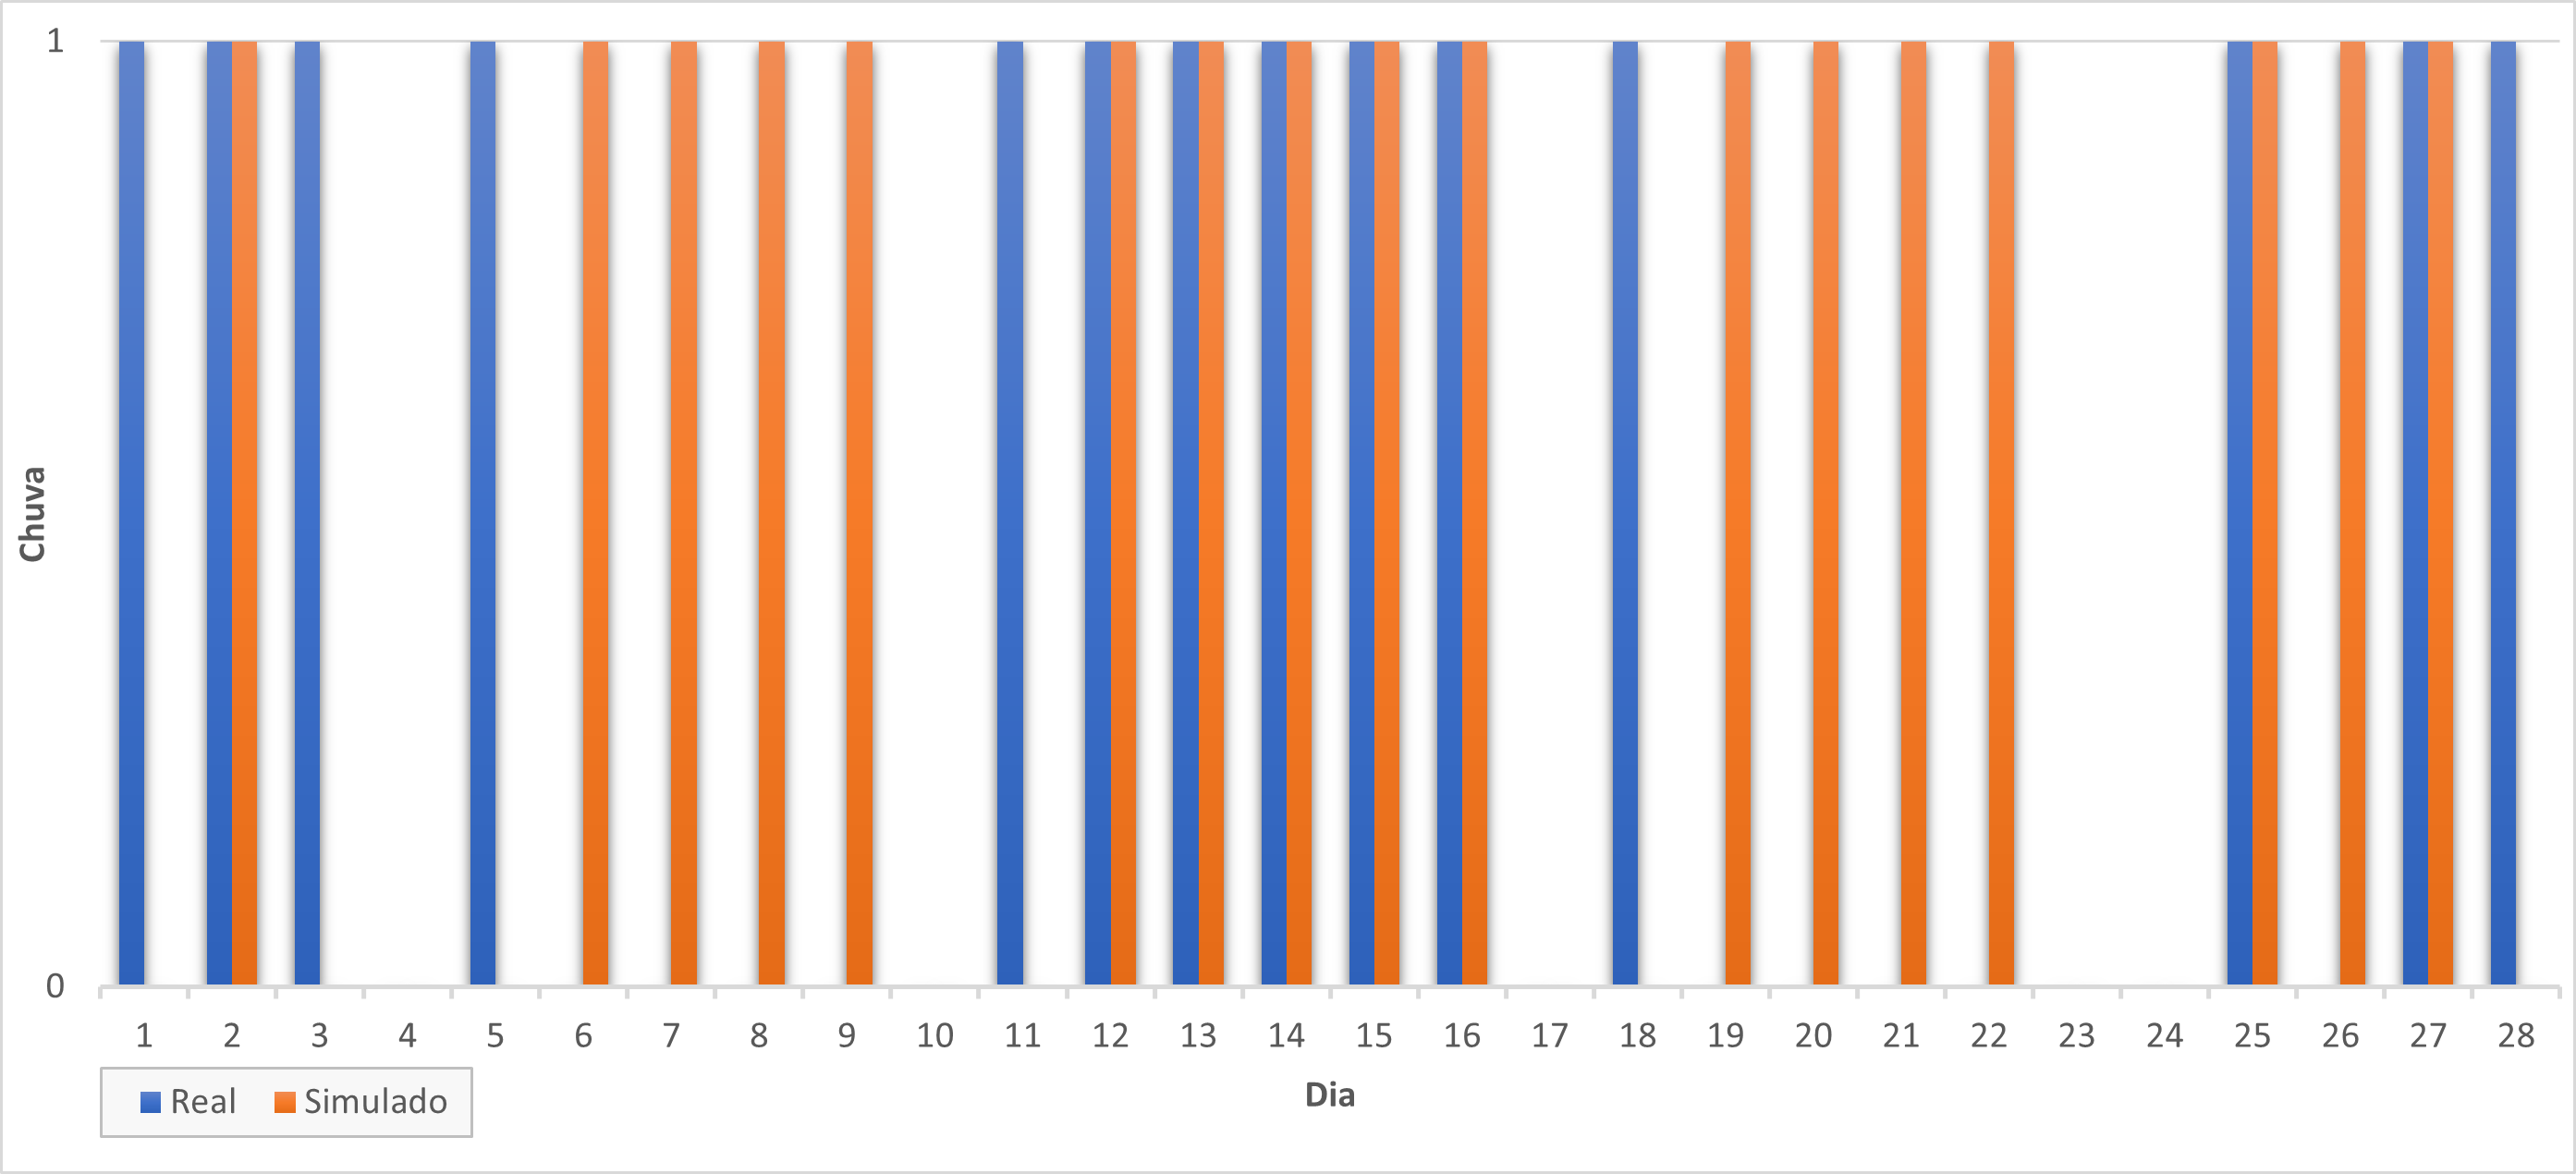
\includegraphics[width=\textwidth]{figs/fev.png}
	\label{f.rfev}
	\legend{\small Fonte: Elaborado pelo autor.}
\end{figure}

\subsection{Marco}
\begin{figure}[H]
	\caption{\small Chuva x Dia - Março/2021}
	\centering
	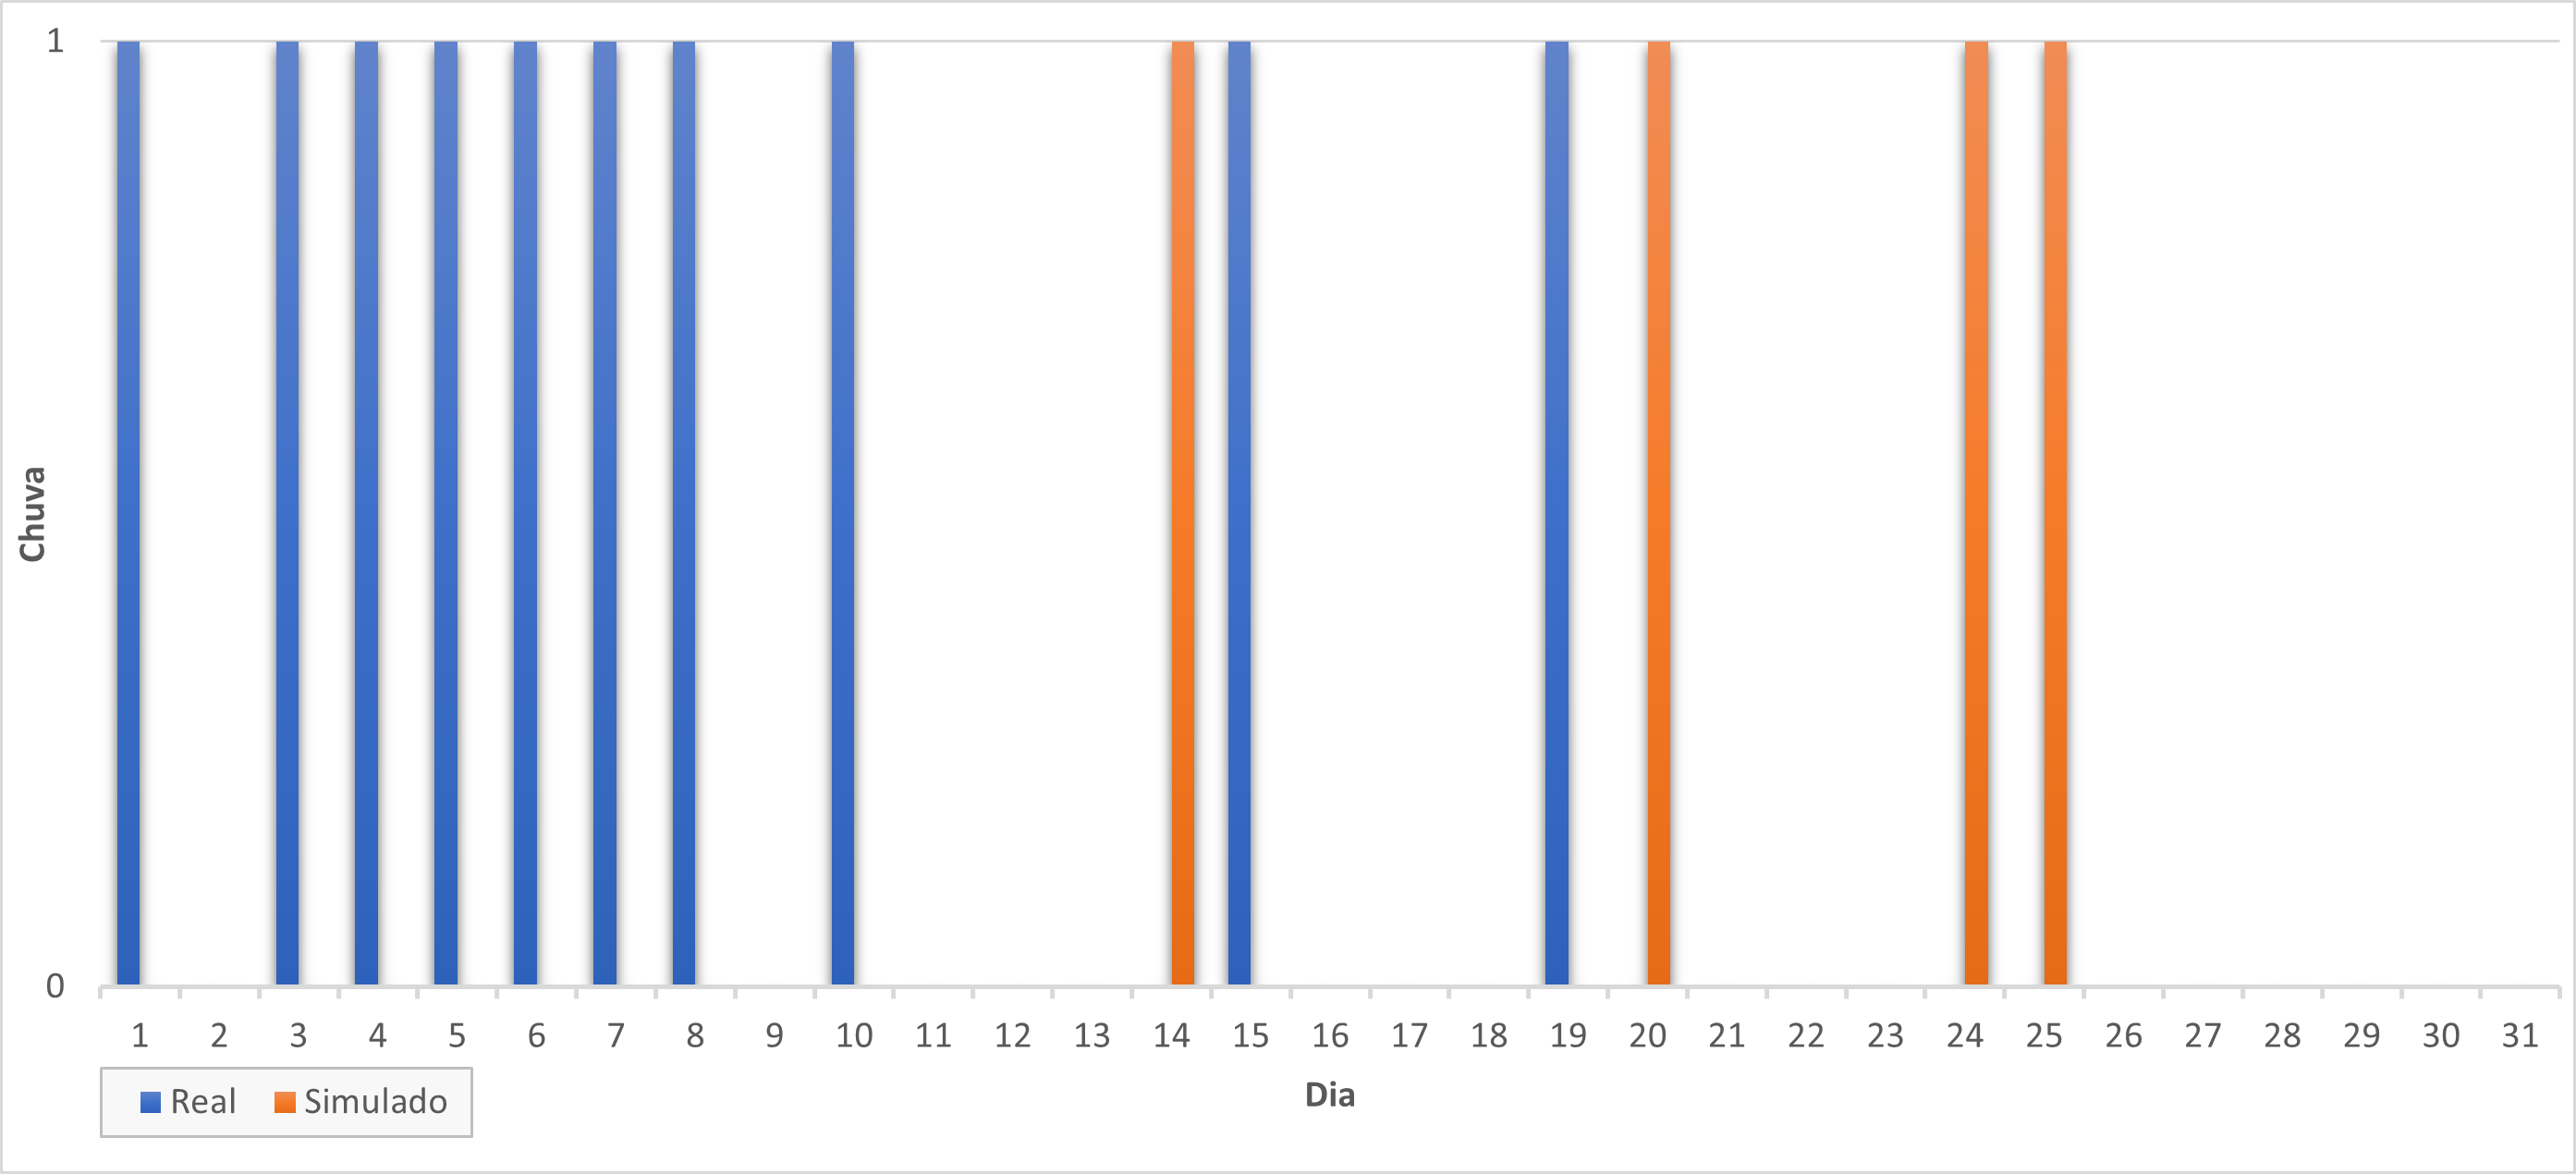
\includegraphics[width=\textwidth]{figs/mar.png}
	\label{f.rmar}
	\legend{\small Fonte: Elaborado pelo autor.}
\end{figure}

\subsection{Abril}
\begin{figure}[H]
	\caption{\small Chuva x Dia - Abril/2021}
	\centering
	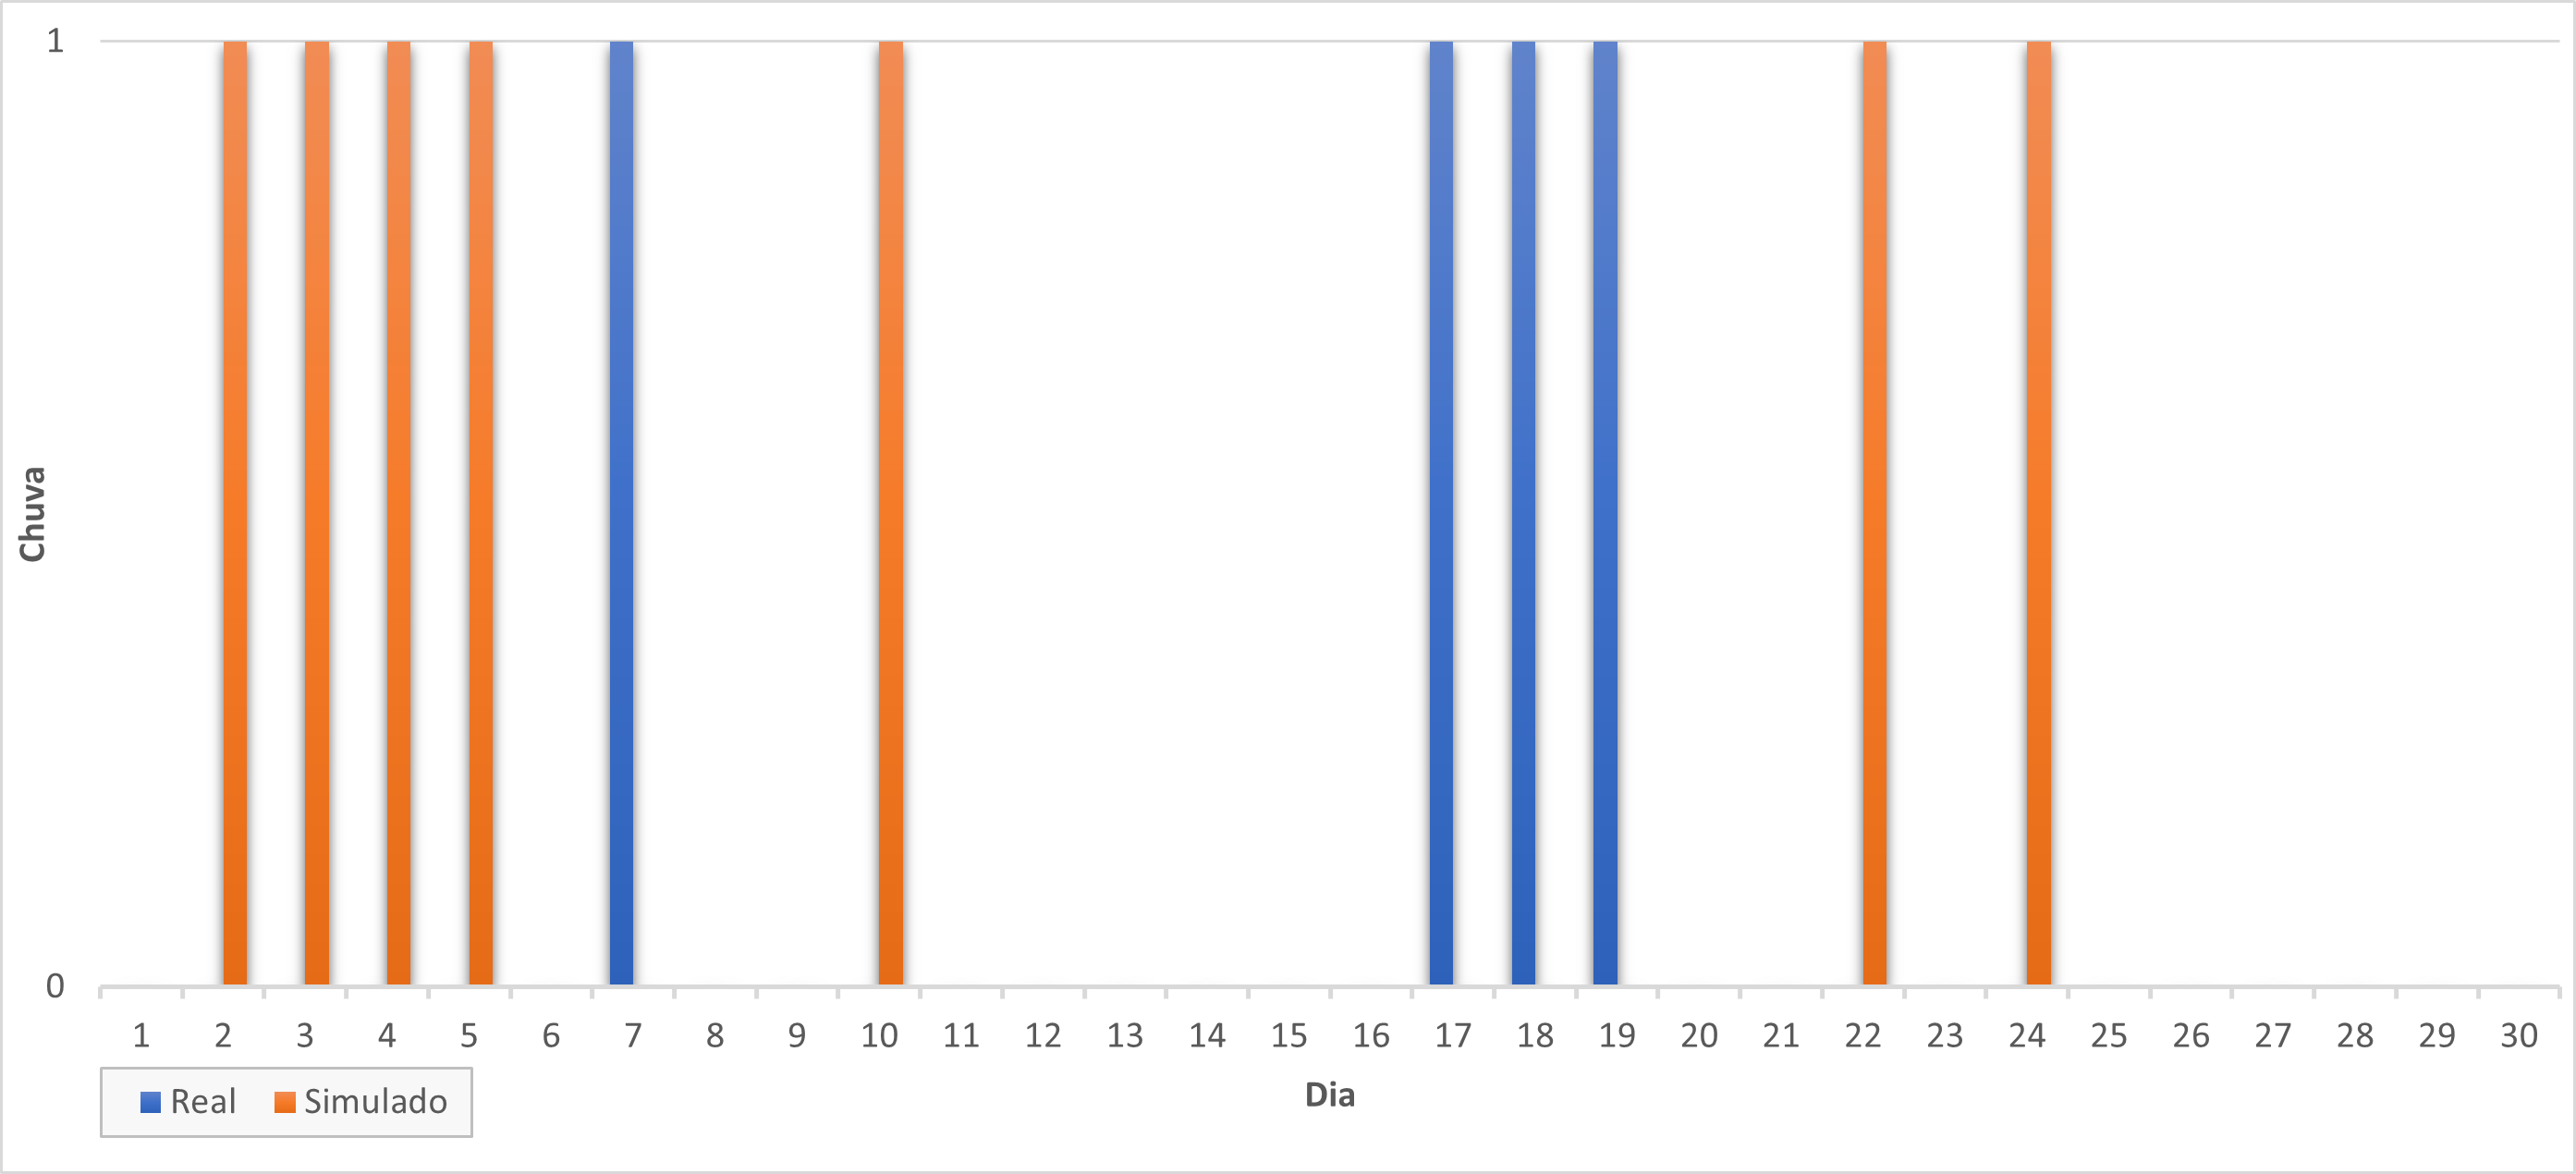
\includegraphics[width=\textwidth]{figs/abr.png}
	\label{f.rabr}
	\legend{\small Fonte: Elaborado pelo autor.}
\end{figure}

\subsection{Maio}
\begin{figure}[H]
	\caption{\small Chuva x Dia - Maio/2021}
	\centering
	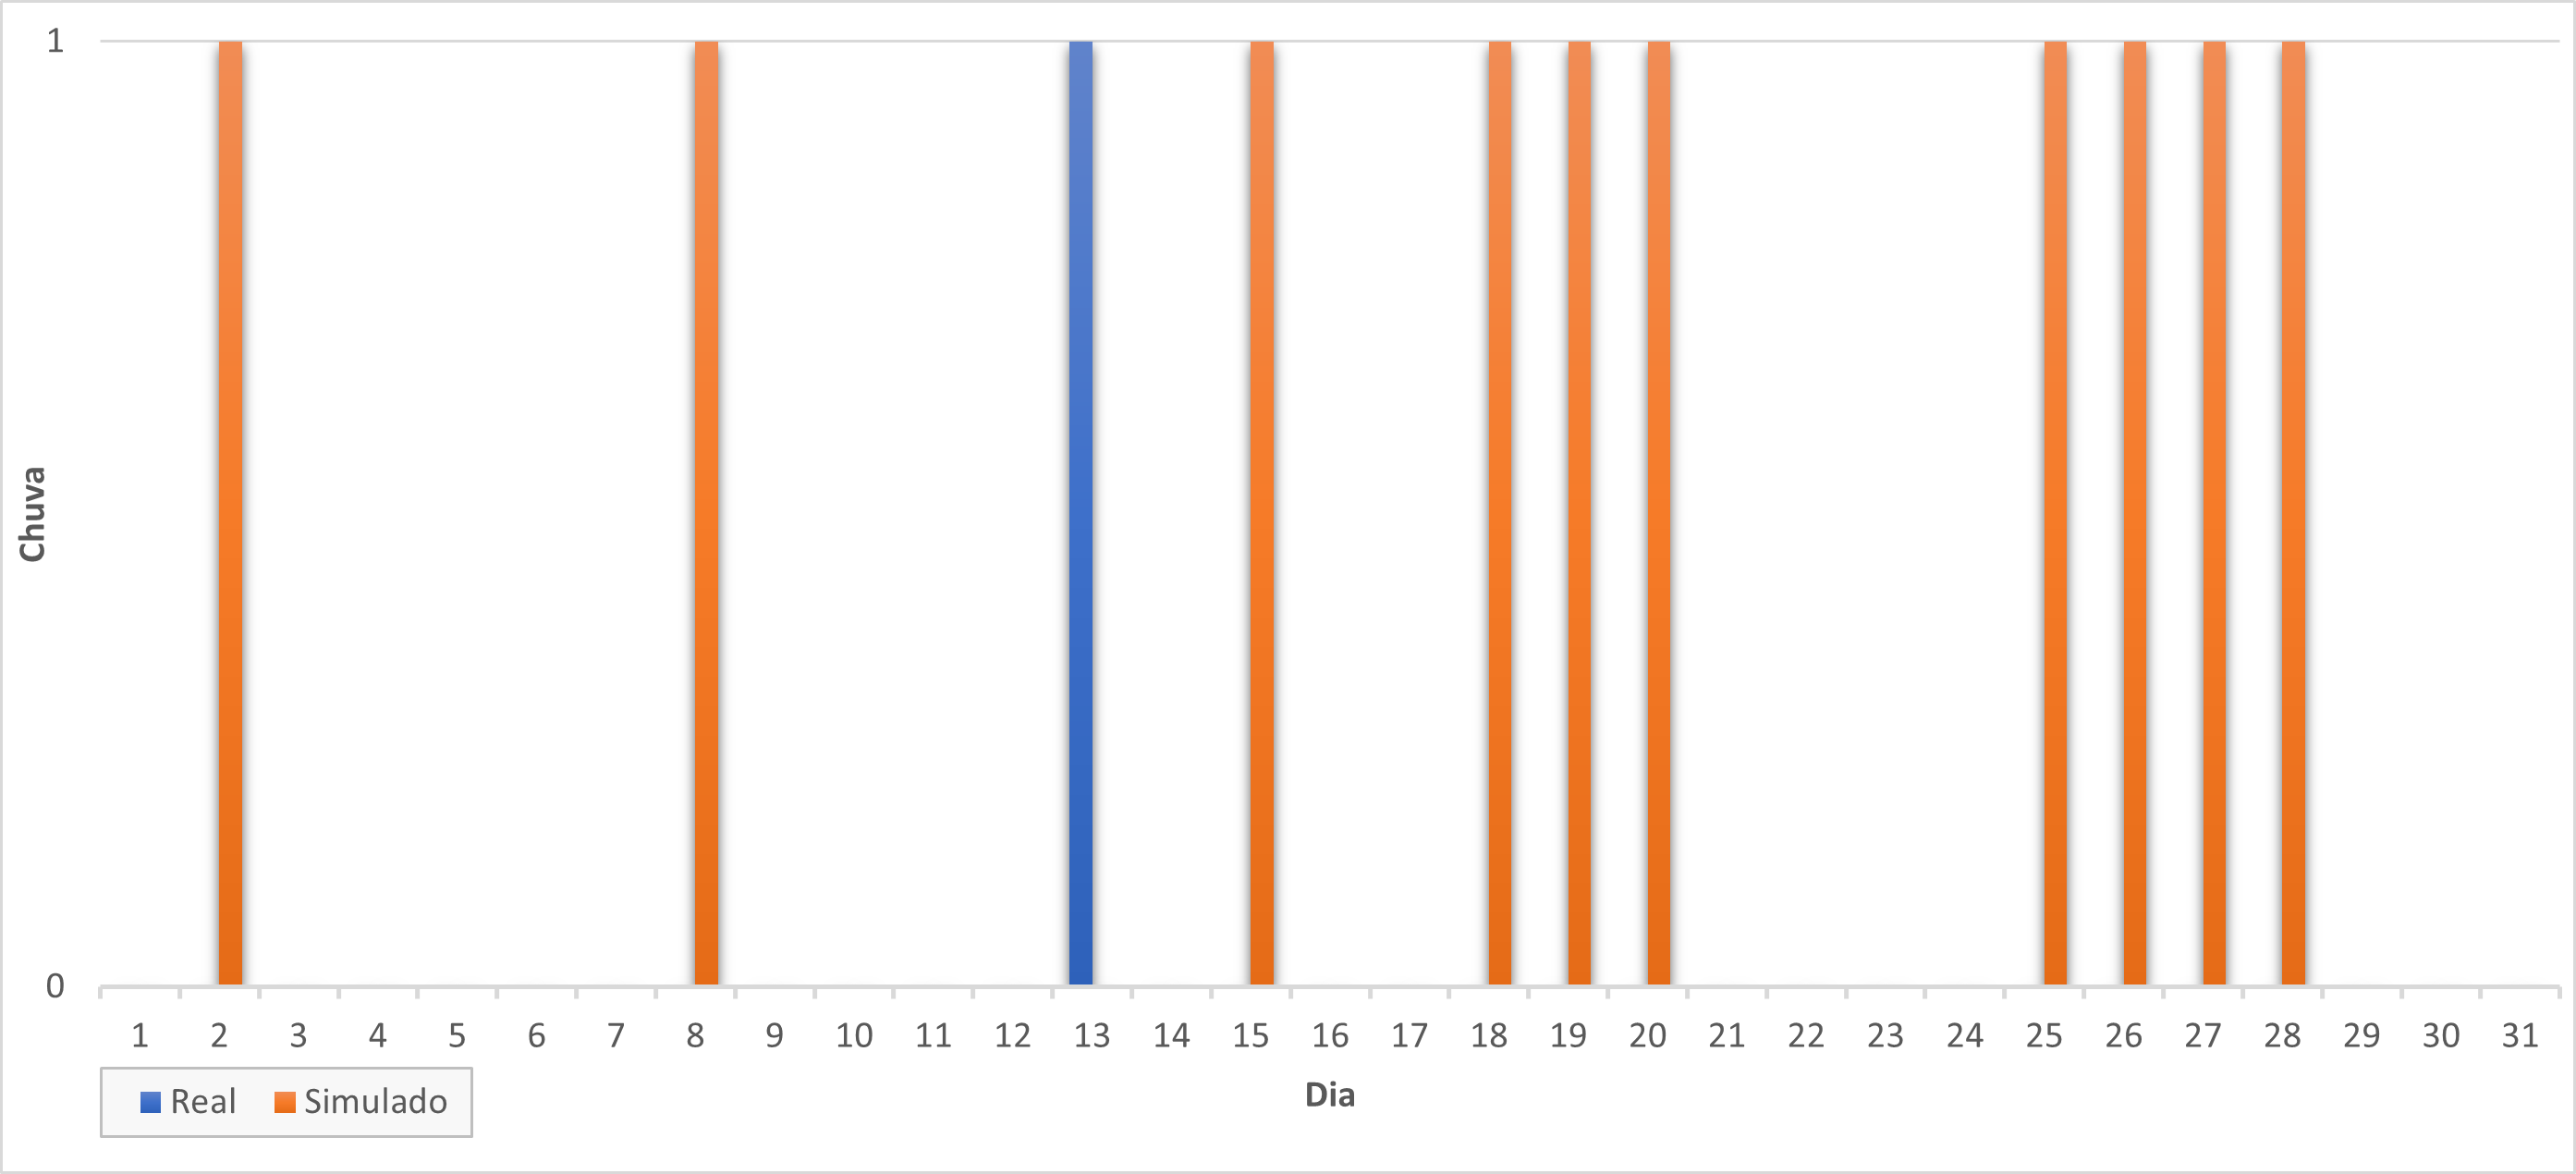
\includegraphics[width=\textwidth]{figs/mai.png}
	\label{f.rmai}
	\legend{\small Fonte: Elaborado pelo autor.}
\end{figure}

\subsection{Junho}
\begin{figure}[H]
	\caption{\small Chuva x Dia - Junho/2021}
	\centering
	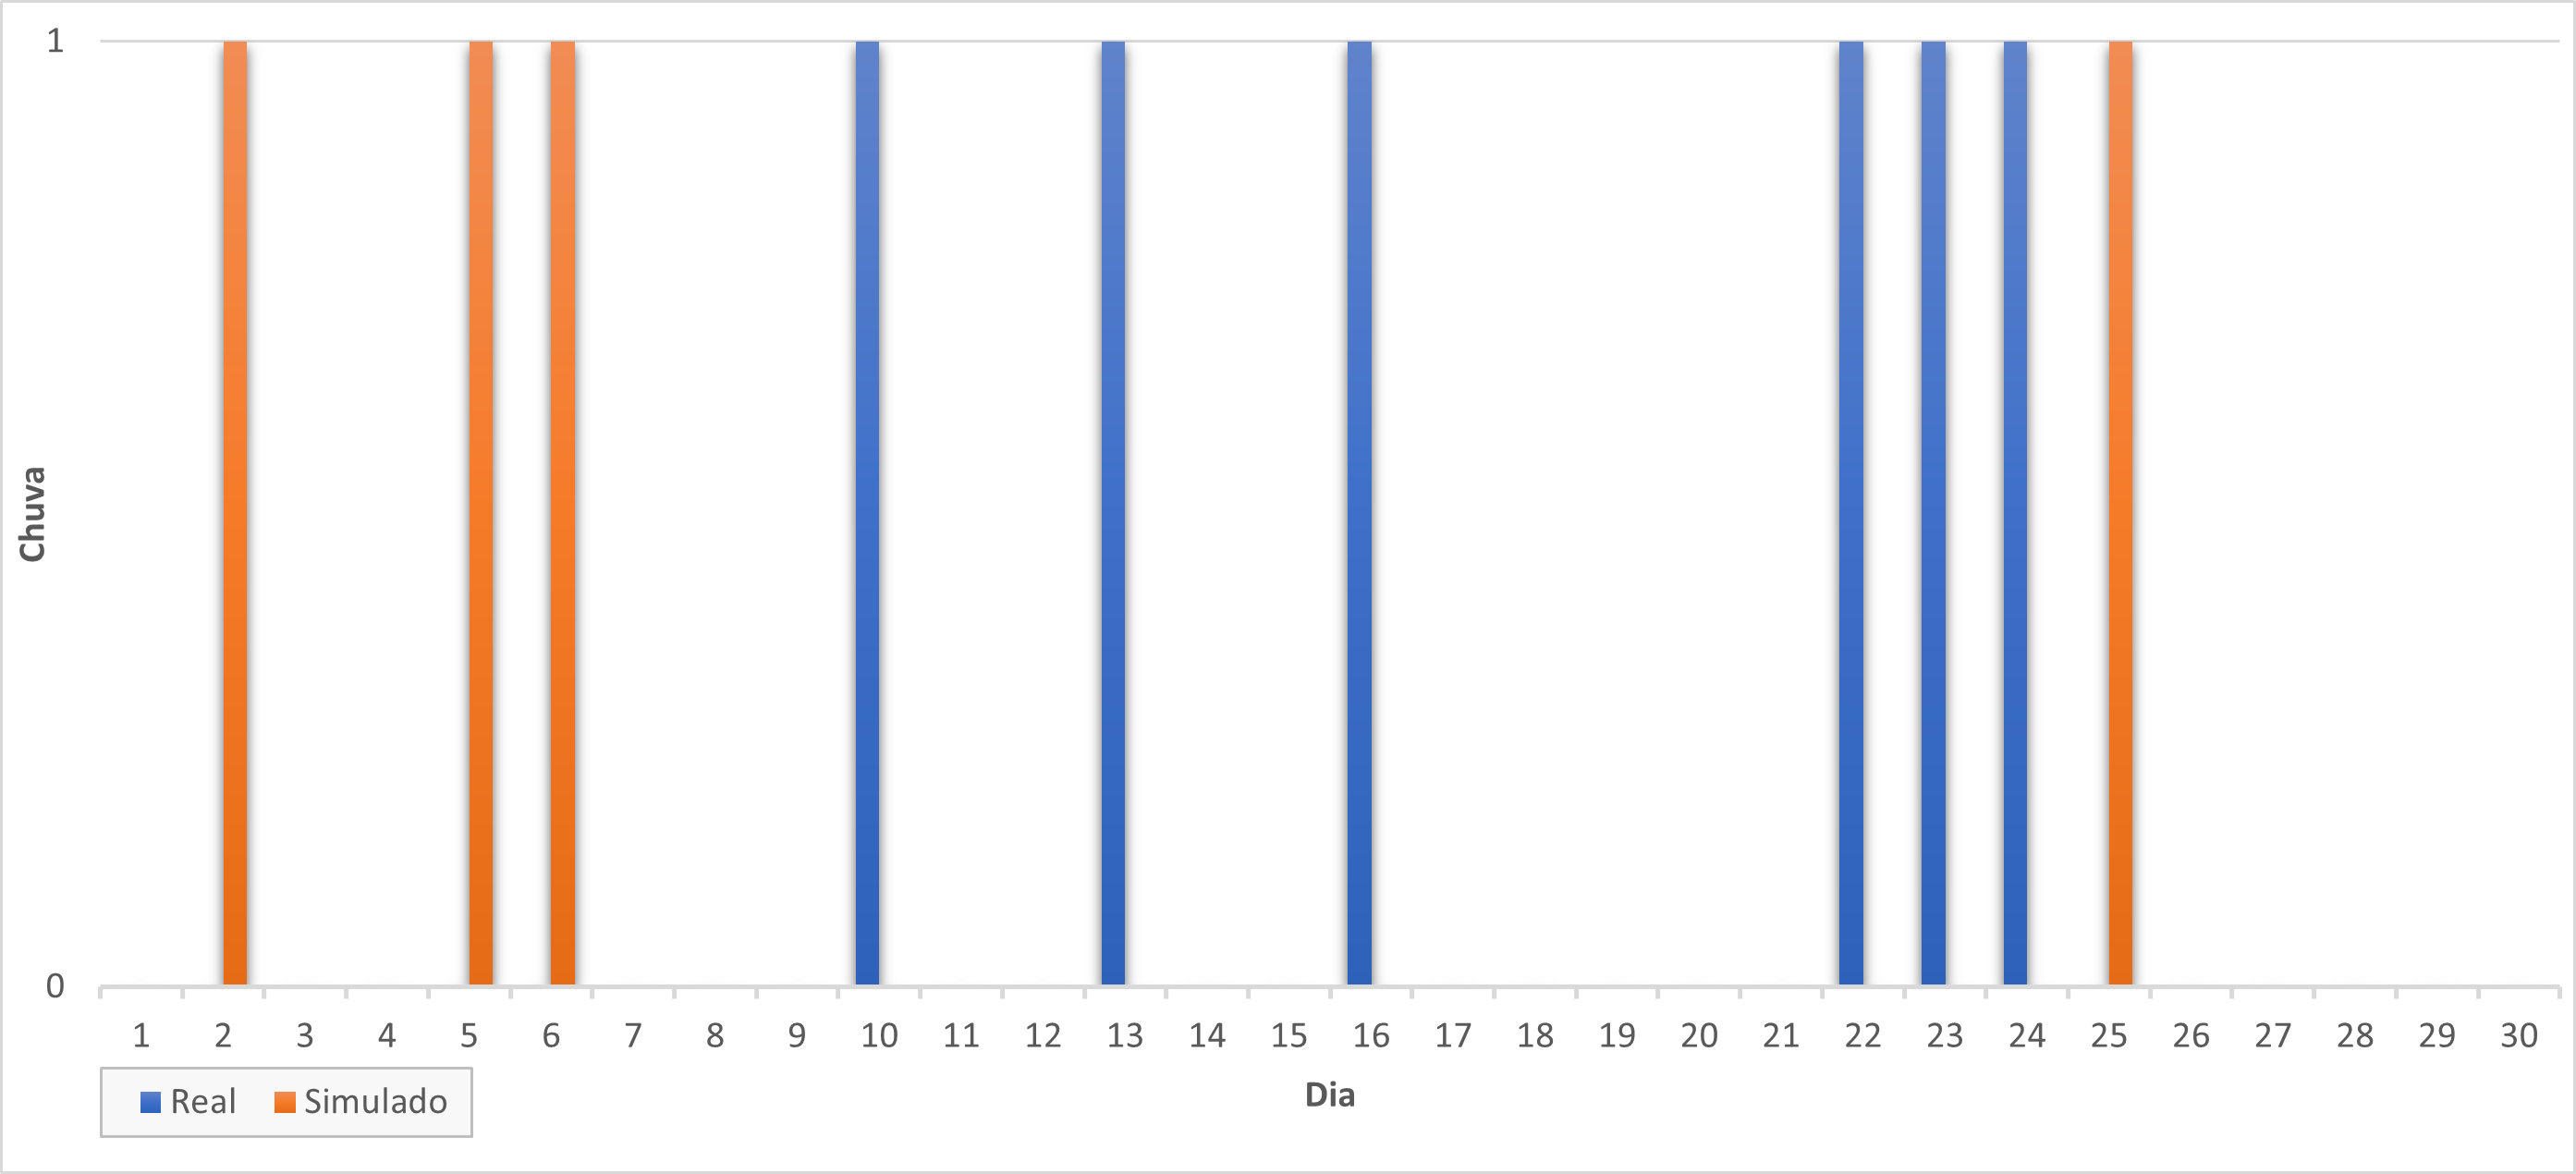
\includegraphics[width=\textwidth]{figs/jun.png}
	\label{f.rjun}
	\legend{\small Fonte: Elaborado pelo autor.}
\end{figure}

\subsection{Julho}
\begin{figure}[H]
	\caption{\small Chuva x Dia - Julho/2021}
	\centering
	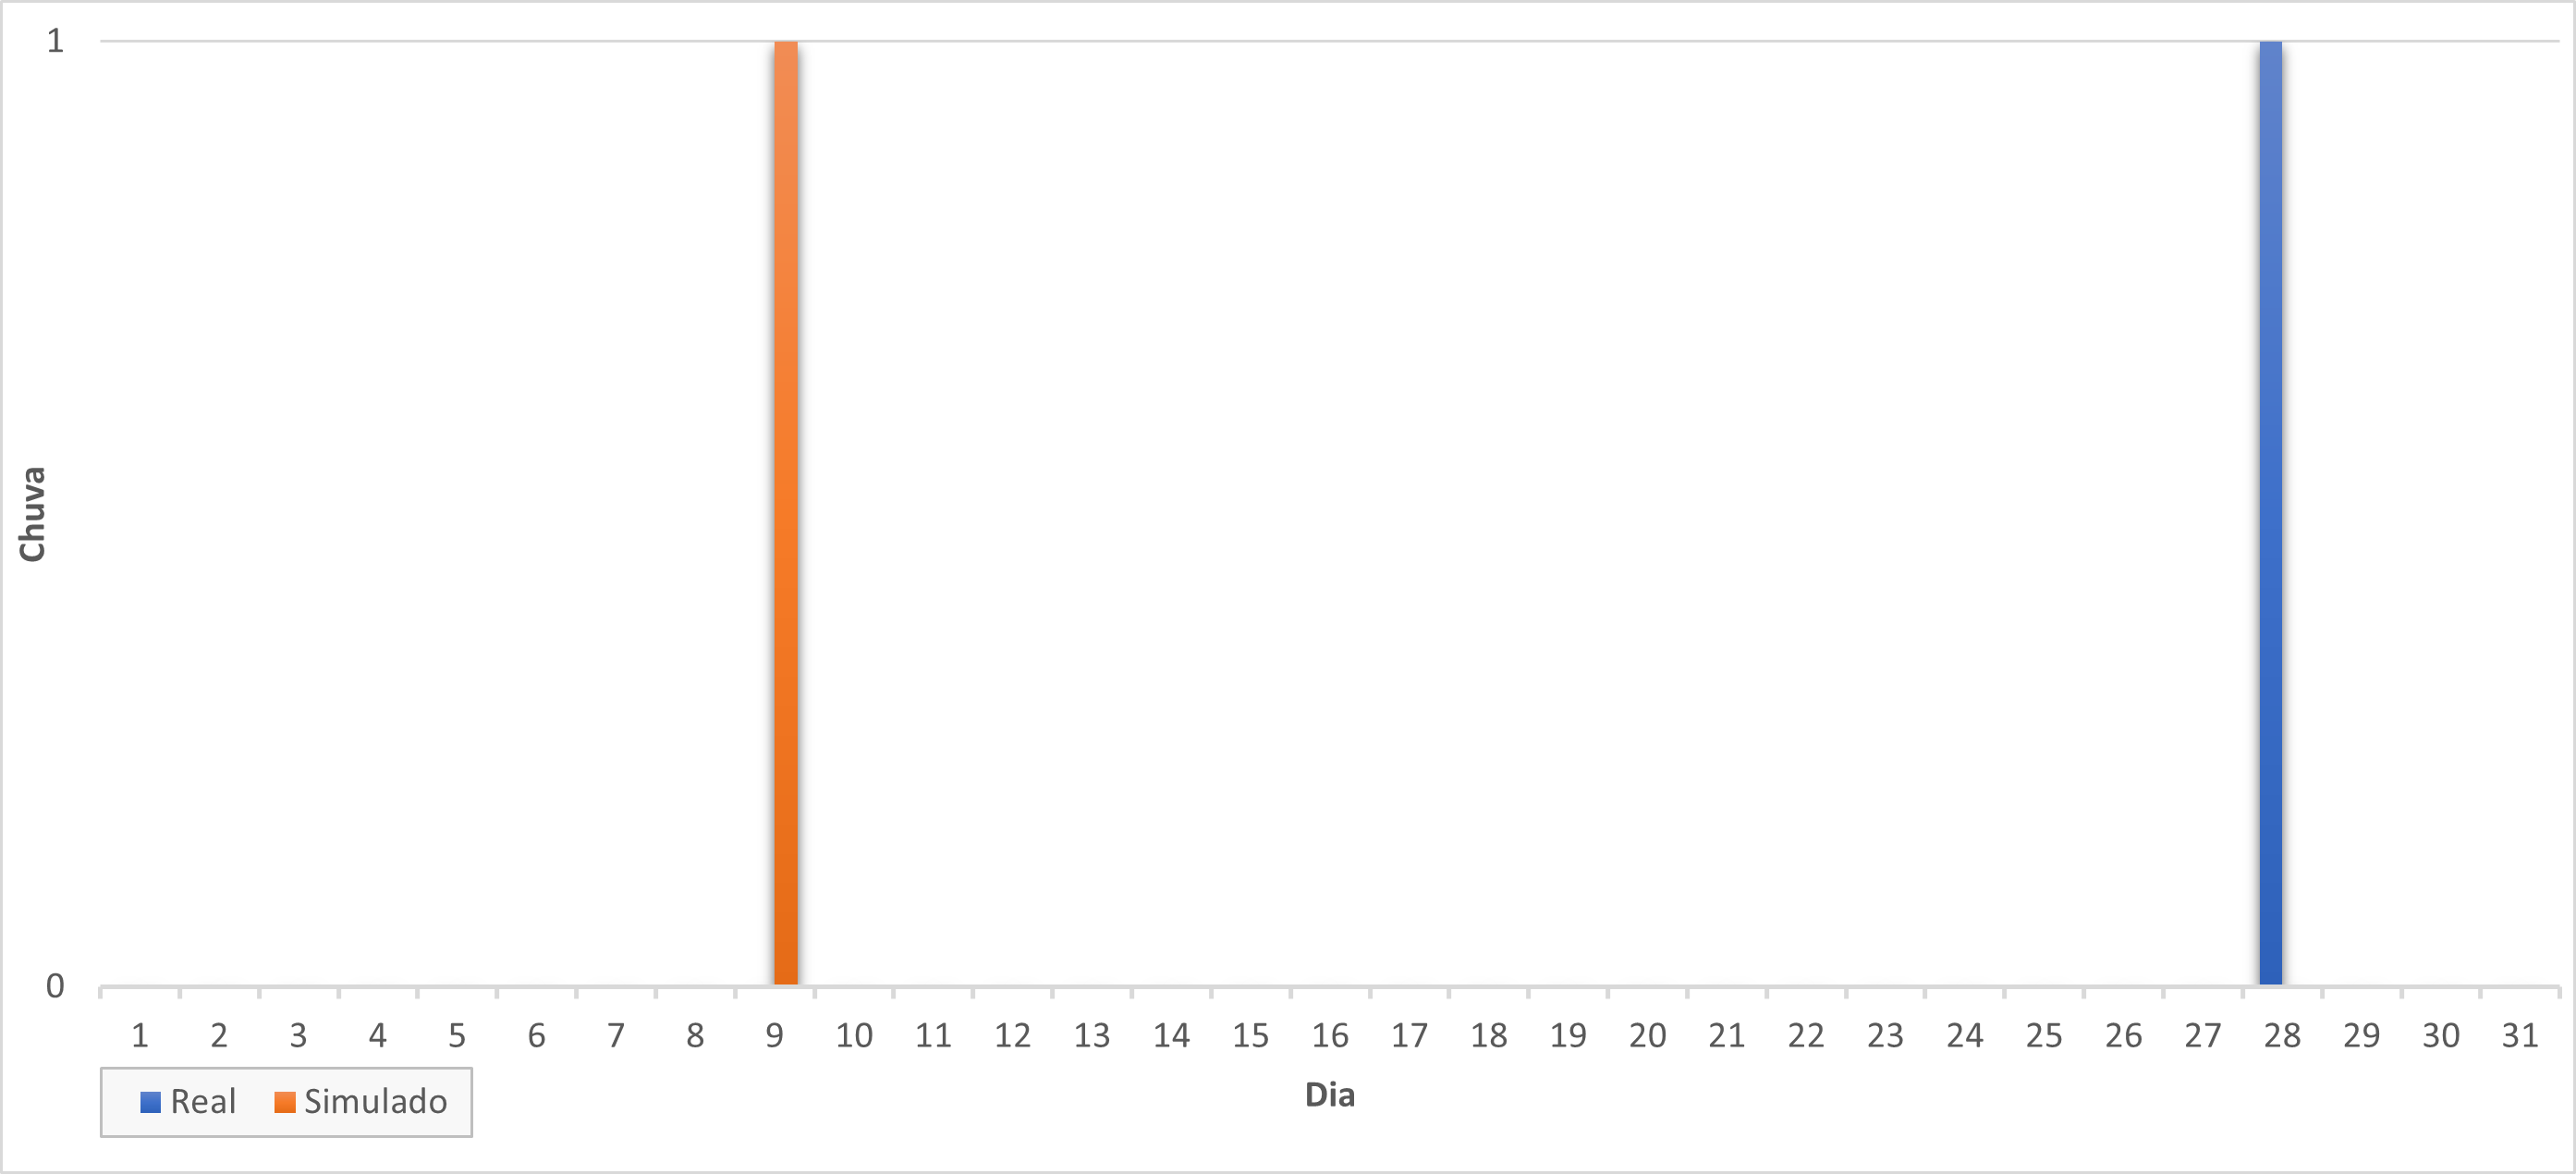
\includegraphics[width=\textwidth]{figs/jul.png}
	\label{f.rjul}
	\legend{\small Fonte: Elaborado pelo autor.}
\end{figure}

\subsection{Agosto}
\begin{figure}[H]
	\caption{\small Chuva x Dia - Agosto/2021}
	\centering
	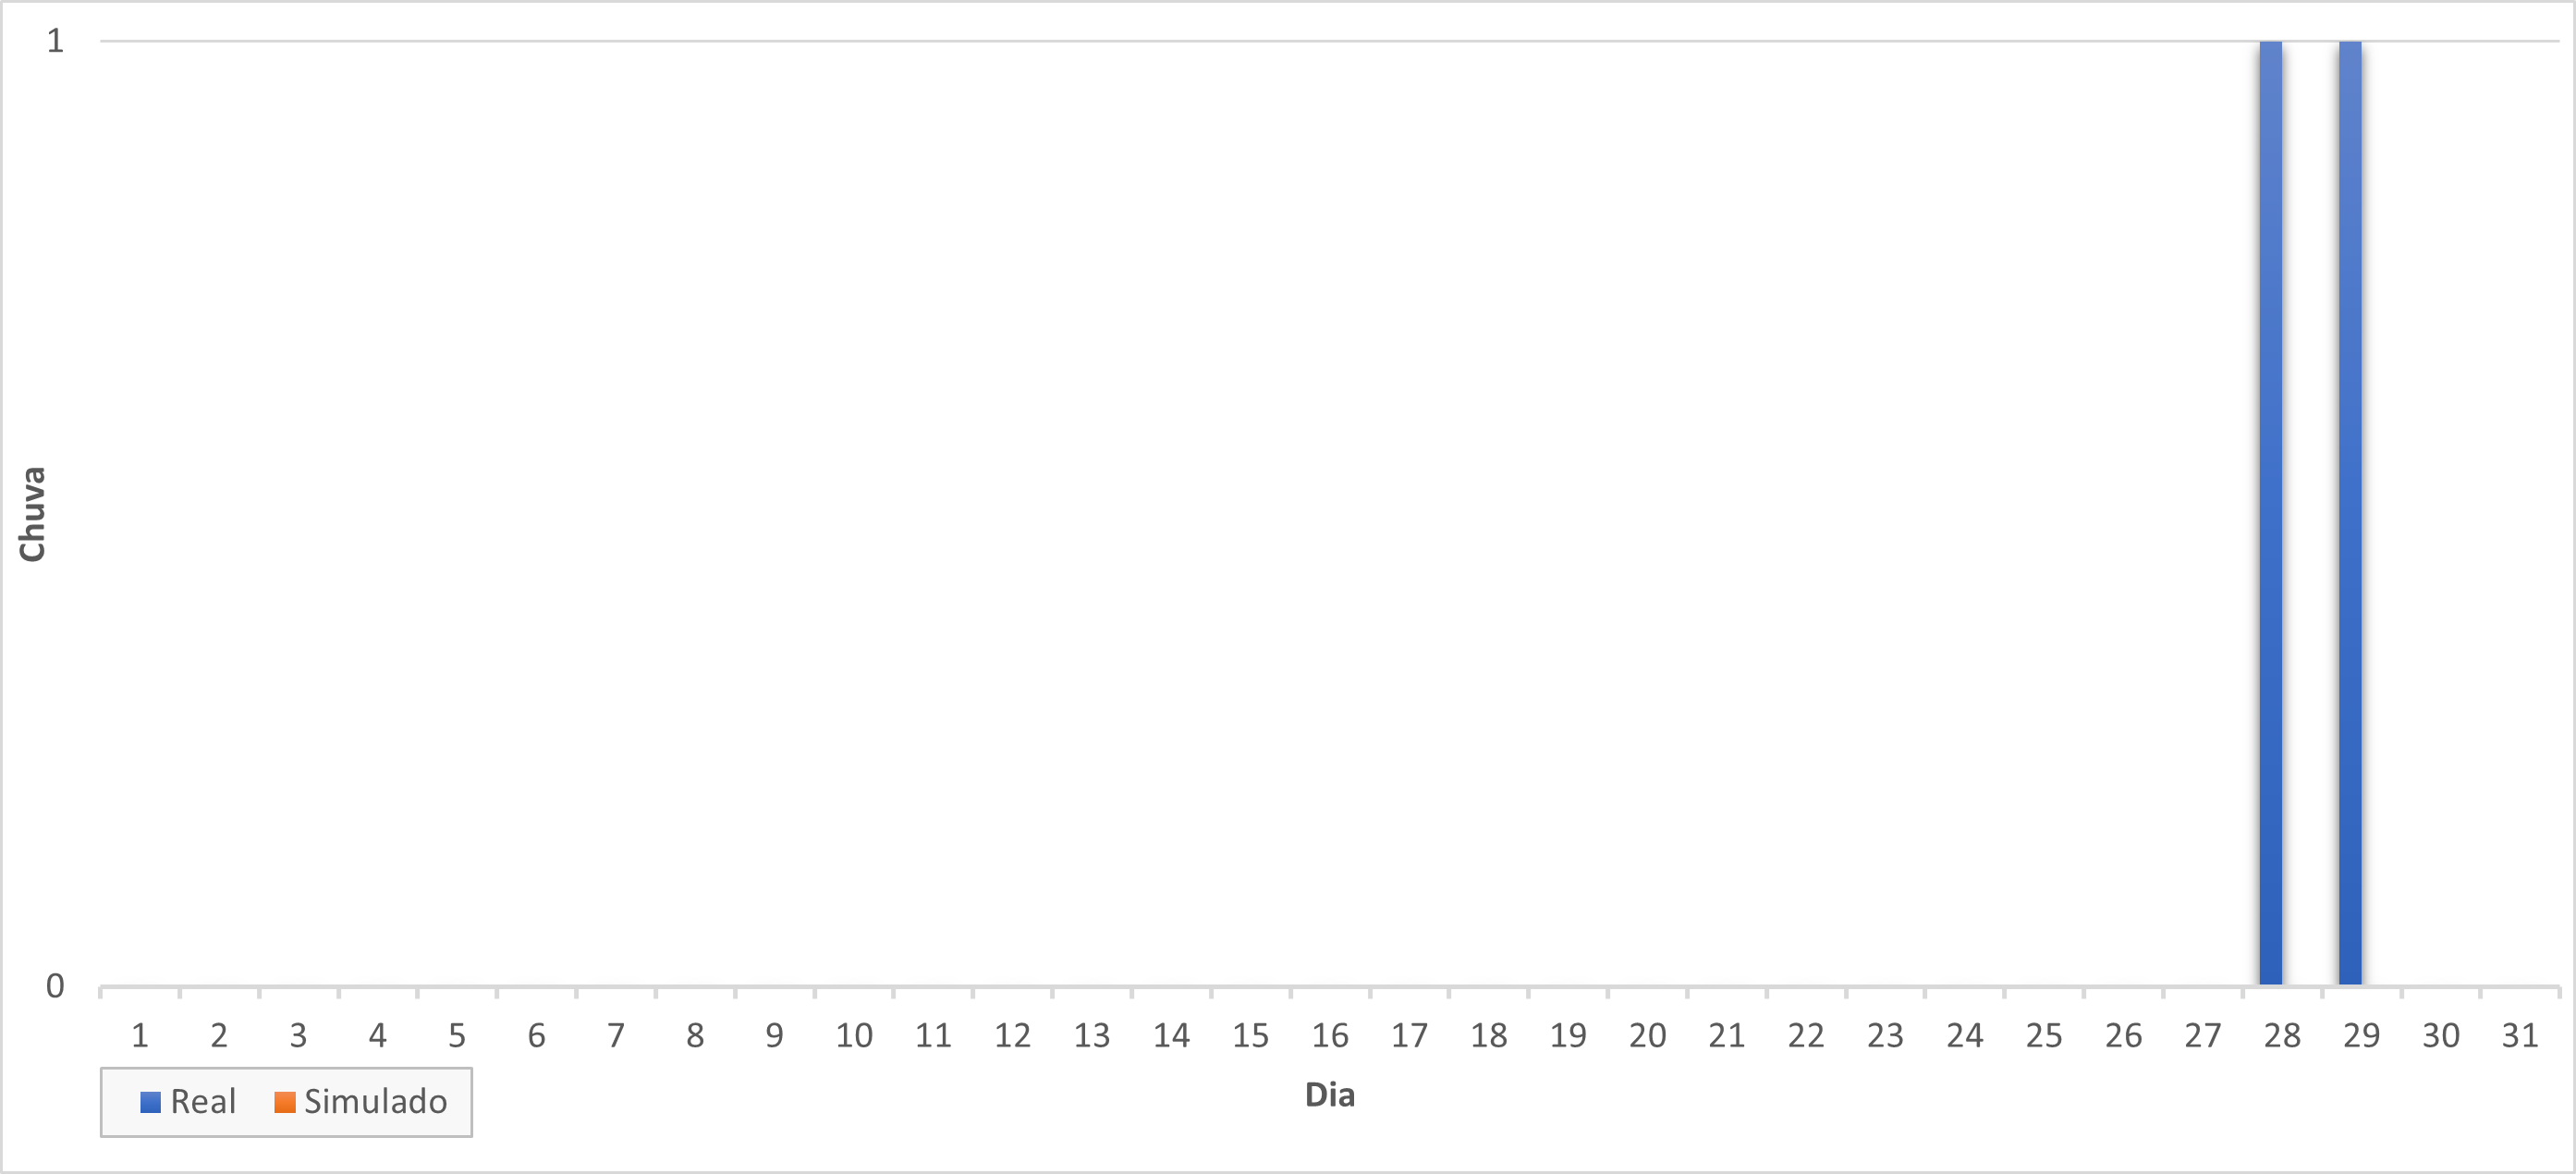
\includegraphics[width=\textwidth]{figs/ago.png}
	\label{f.rago}
	\legend{\small Fonte: Elaborado pelo autor.}
\end{figure}

\subsection{Setembro}
\begin{figure}[H]
	\caption{\small Chuva x Dia - Setembro/2021}
	\centering
	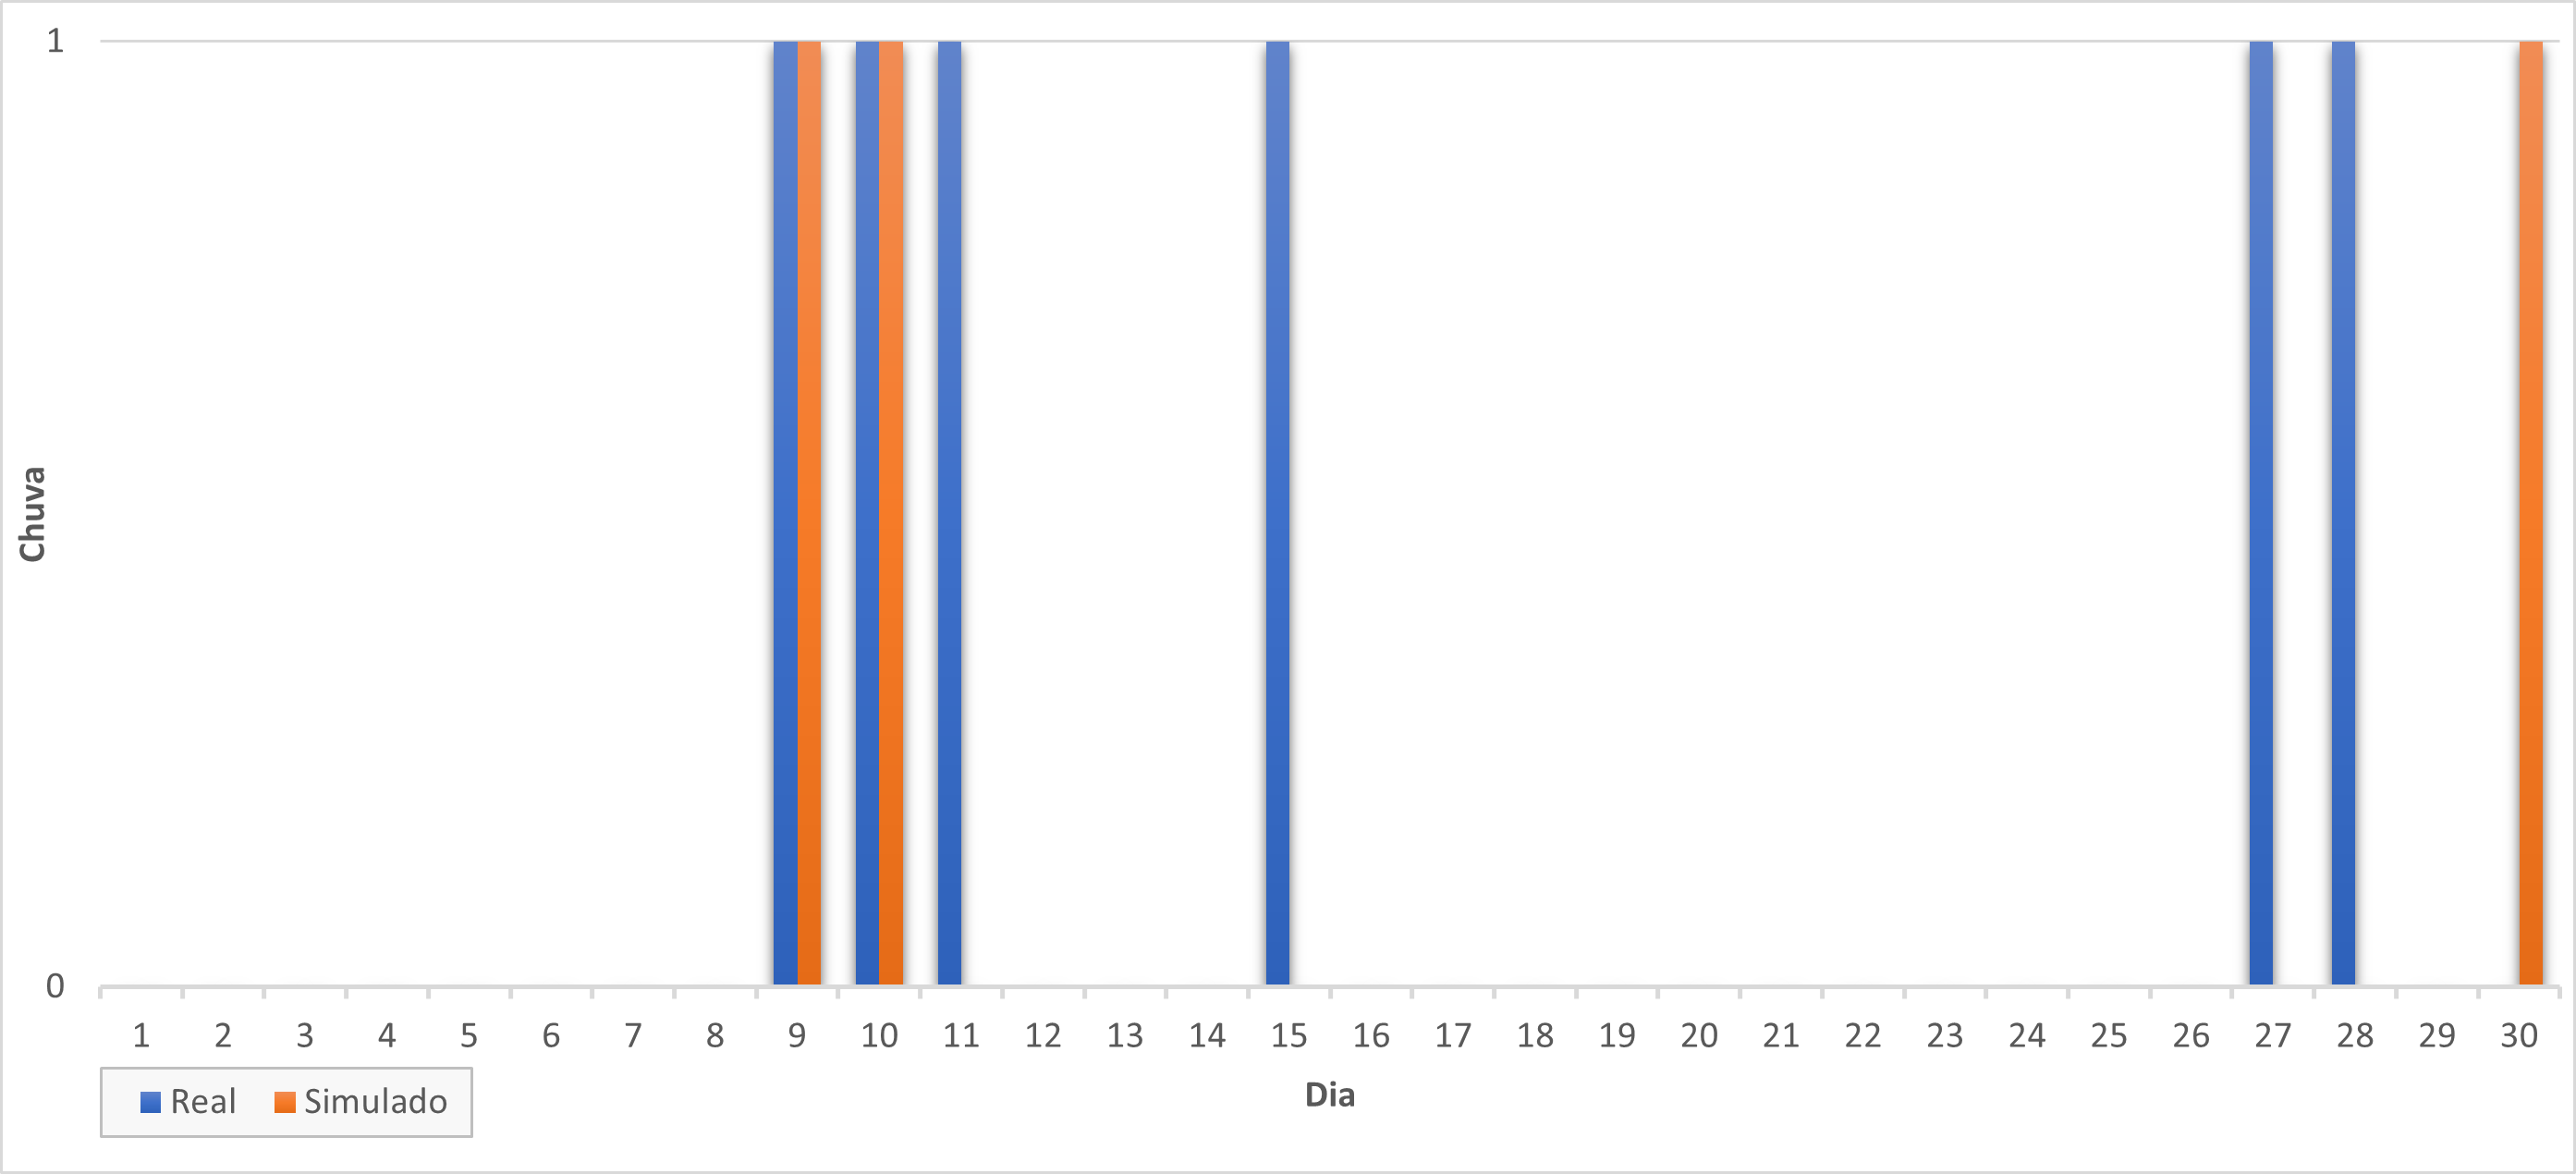
\includegraphics[width=\textwidth]{figs/set.png}
	\label{f.rset}
	\legend{\small Fonte: Elaborado pelo autor.}
\end{figure}

\subsection{Outubro}
\begin{figure}[H]
	\caption{\small Chuva x Dia - Outubro/2021}
	\centering
	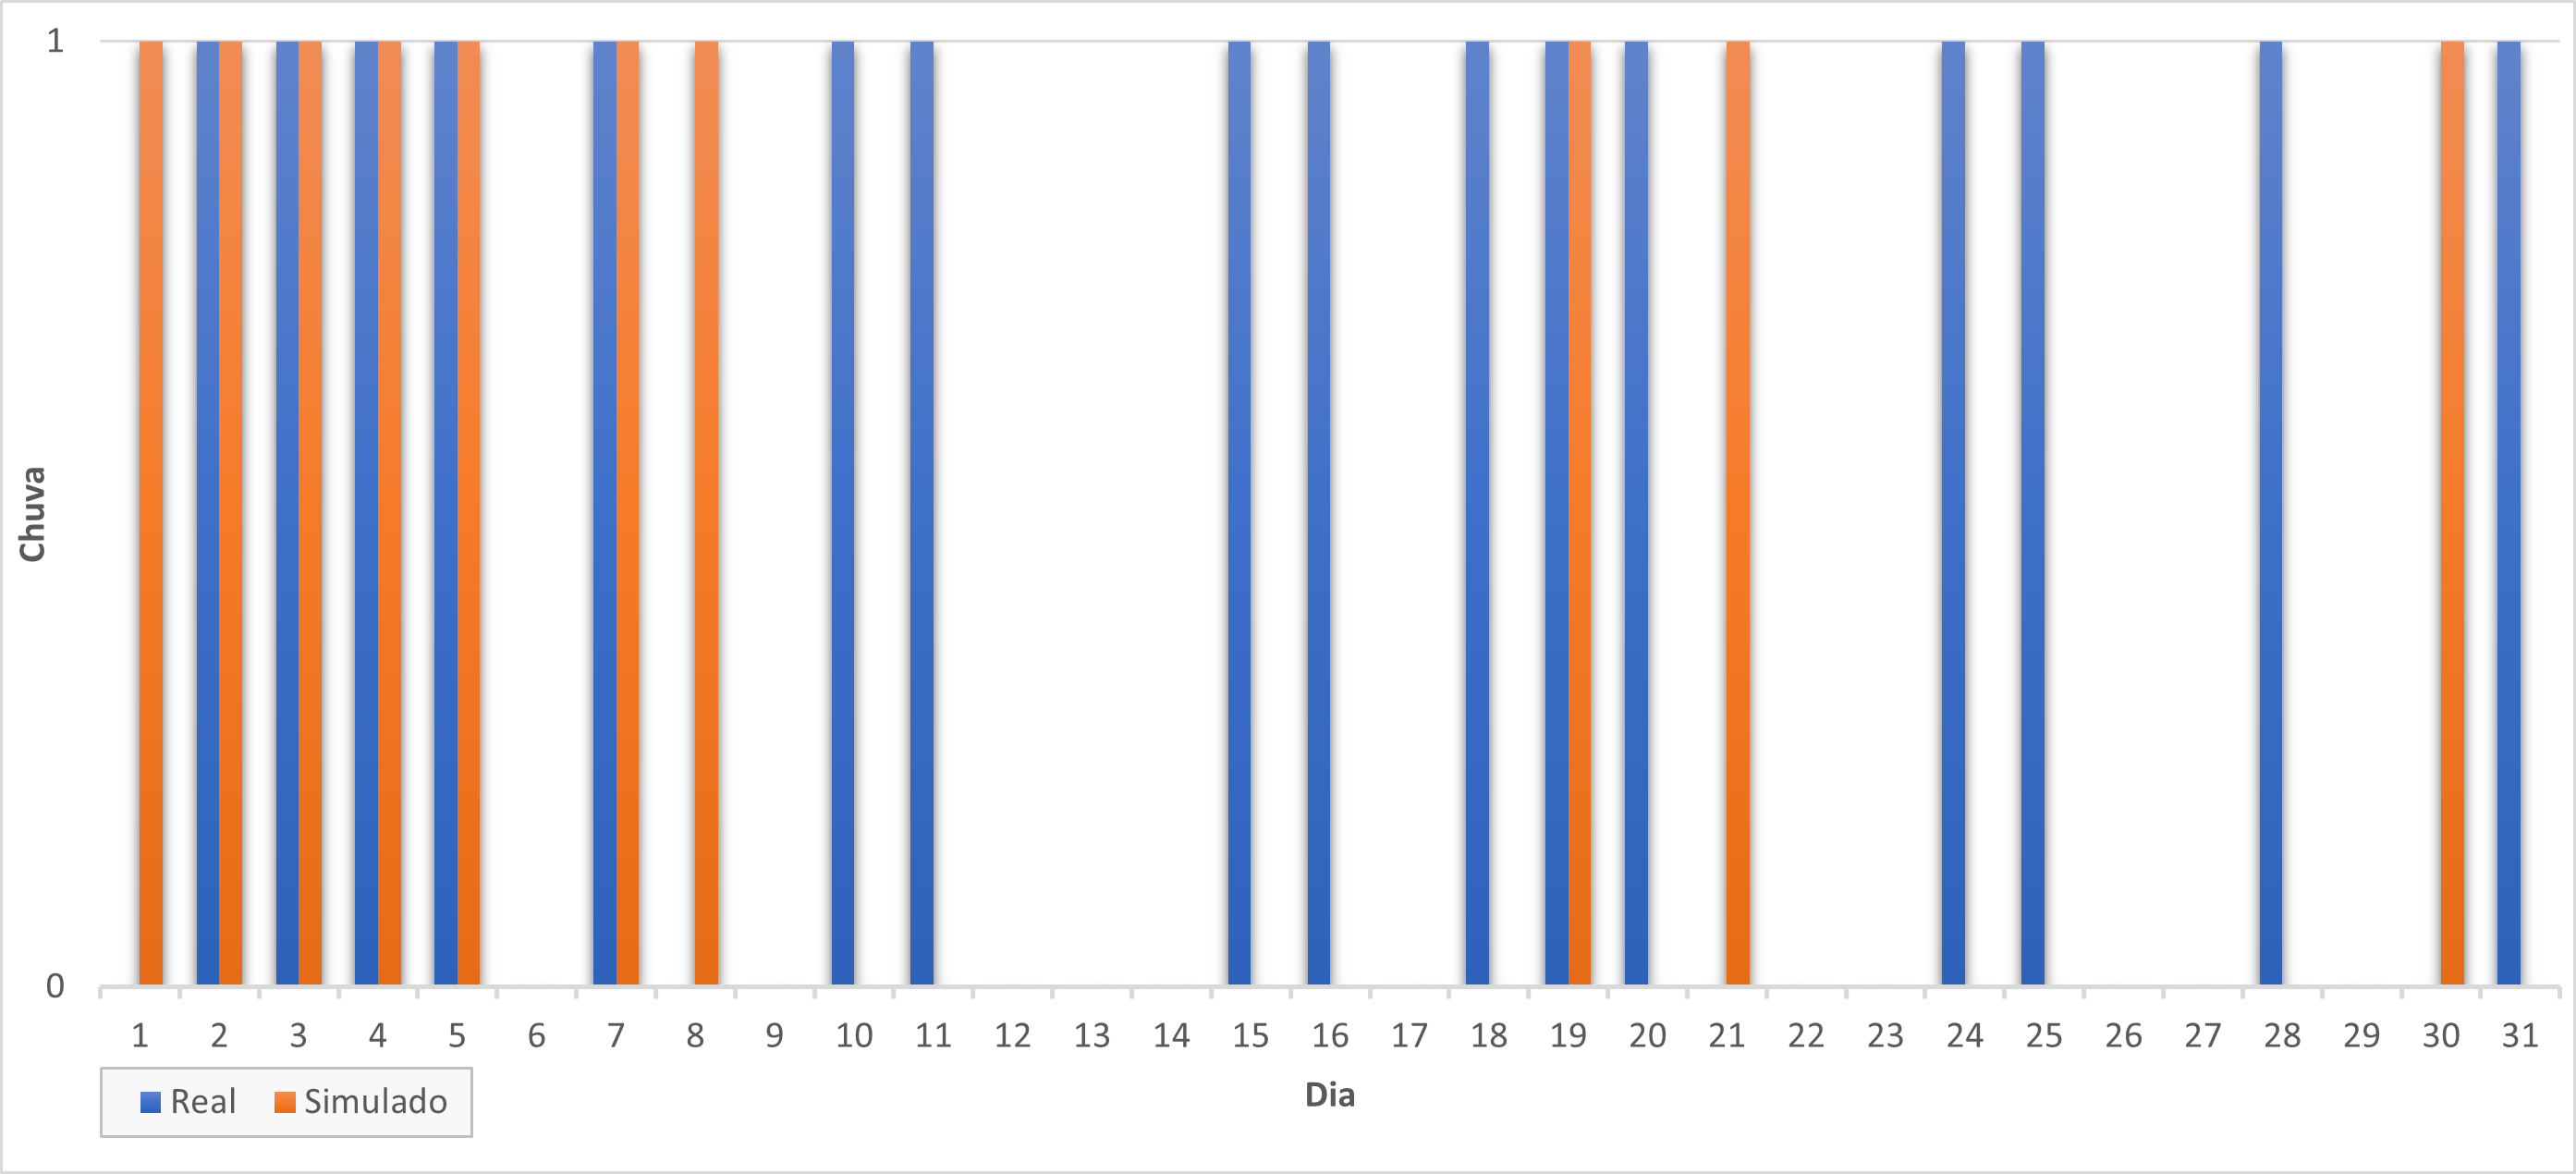
\includegraphics[width=\textwidth]{figs/out.png}
	\label{f.rout}
	\legend{\small Fonte: Elaborado pelo autor.}
\end{figure}

\subsection{Novembro}
\begin{figure}[H]
	\caption{\small Chuva x Dia - Novembro/2021}
	\centering
	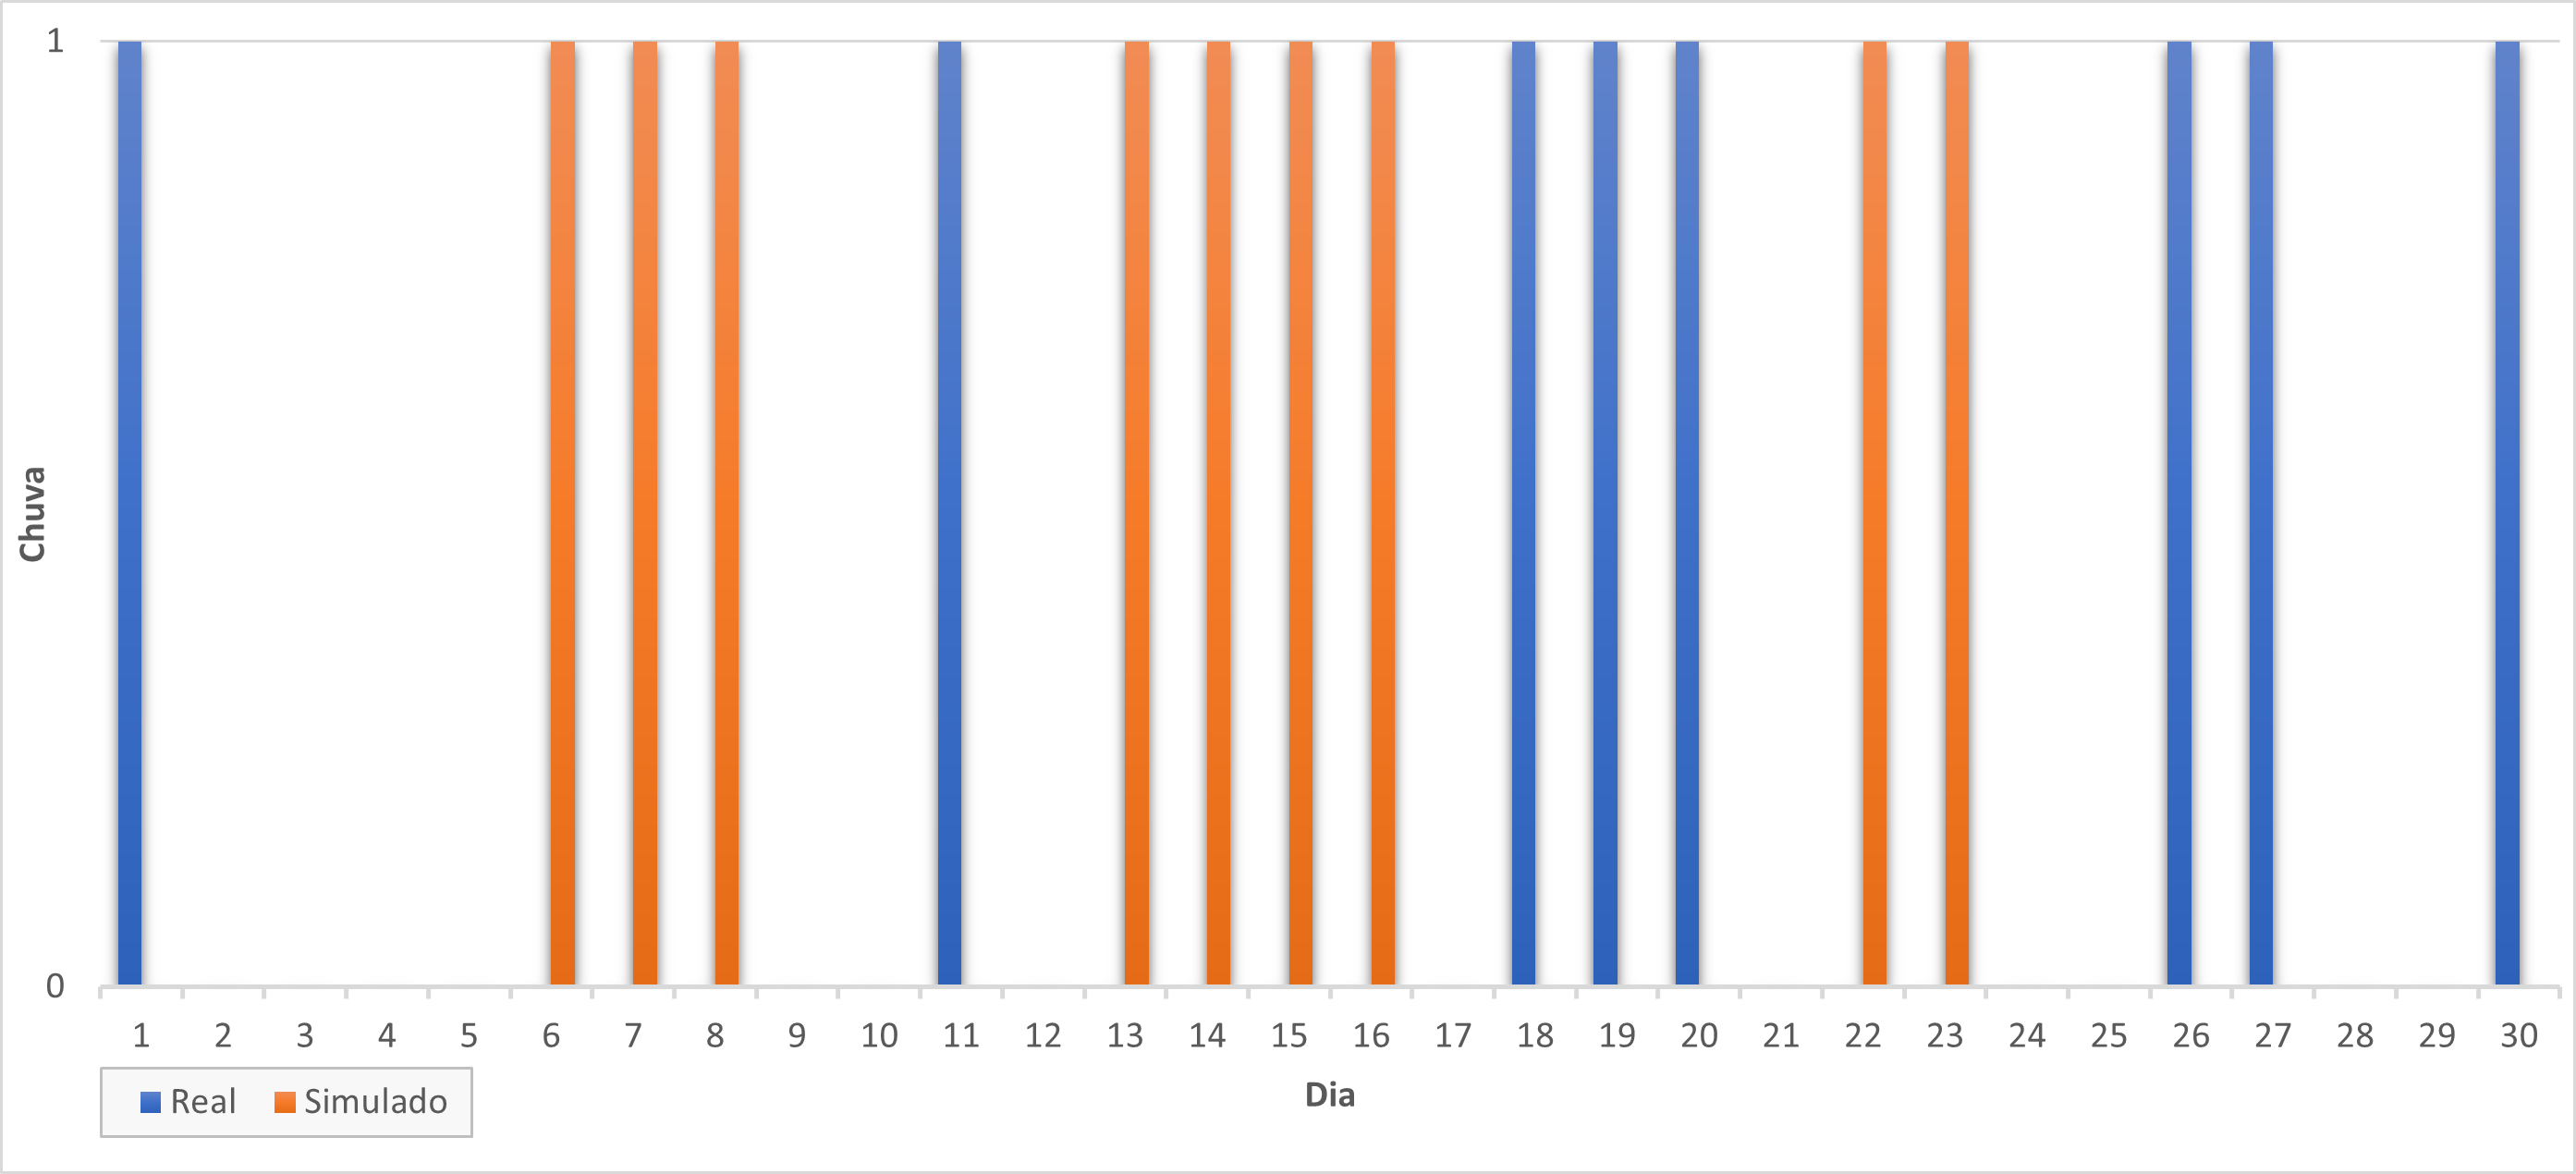
\includegraphics[width=\textwidth]{figs/nov.png}
	\label{f.rnov}
	\legend{\small Fonte: Elaborado pelo autor.}
\end{figure}

\subsection{Dezembro}
\begin{figure}[H]
	\caption{\small Chuva x Dia - Dezembro/2021}
	\centering
	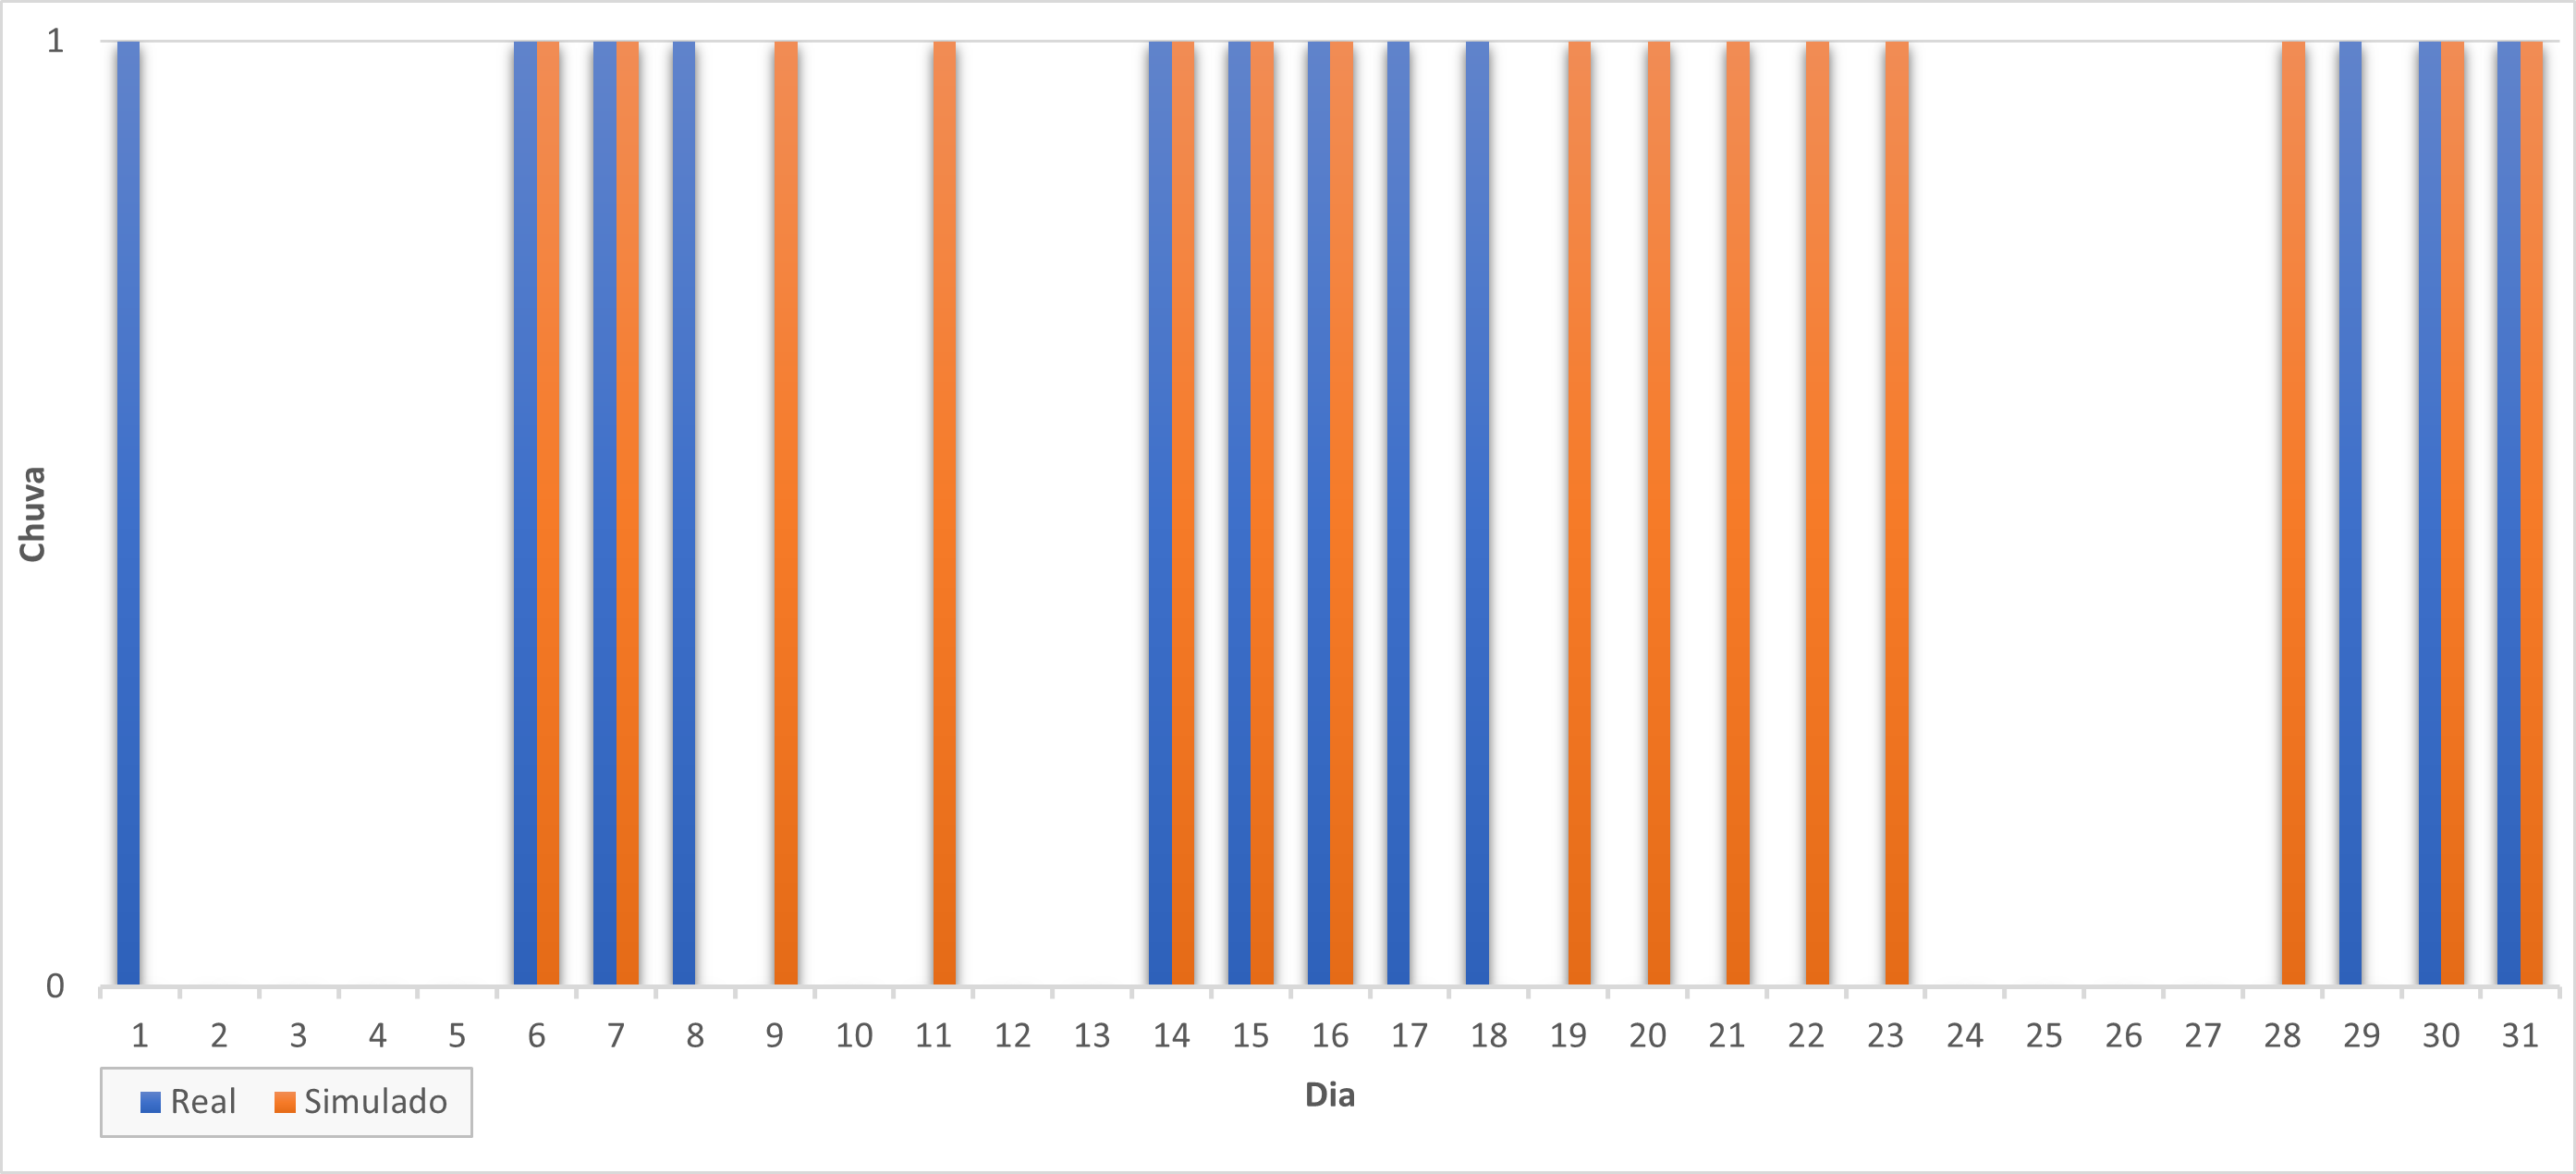
\includegraphics[width=\textwidth]{figs/dez.png}
	\label{f.rdez}
	\legend{\small Fonte: Elaborado pelo autor.}
\end{figure}


\section{Análise do ano inteiro}
\chapter{Conclusão}
\label{c.conclusao}



\section{Desafios Encontrados}
\label{s.desafios}
E interessante introduzir tecnologias novas, mais especificamente na área da meteorologia, onde já existem algumas soluções extremamente precisas. Desenvolver uma abordagem alternativa e inovadora para a solução do problema que será explicado na próxima sessão deve ter no mínimo um bom grau de precisão para que possa ter algum uso na agronomia ou áreas afins.

\section{Aspectos Positivos}
\label{s.aspectos}

\section{Projetos Futuros}
\label{s.projetos}


% --------------------------------------------------------
% ELEMENTOS PÓS-TEXTUAIS
% --------------------------------------------------------

\postextual


% --------------------------------------------------------
% REFERÊNCIAS BIBLIOGRÁFICAS
% --------------------------------------------------------

\bibliography{chapters/referencias}


% --------------------------------------------------------
% GLOSSÁRIO
% --------------------------------------------------------

% Consulte o manual da classe abntex2 para orientações sobre o glossário.
%\glossary


% --------------------------------------------------------
% APÊNDICES
% --------------------------------------------------------

% Inicia os apêndices
%\begin{apendicesenv}
% Imprime uma página indicando o início dos apêndices
%\partapendices
% Criação do apêndice
%\end{apendicesenv}


% --------------------------------------------------------
% ÍNDICE REMISSIVO
% --------------------------------------------------------

%\printindex


% --------------------------------------------------------
% FINAL DO DOCUMENTO
% --------------------------------------------------------

\end{document}